% shtthesis, an unofficial LaTeX thesis template for ShanghaiTech University.
% Copyright (C) 2022 Li Rundong <rundong.001@gmail.com>
%
% This program is free software: you can redistribute it and/or modify
% it under the terms of the GNU General Public License as published by
% the Free Software Foundation, either version 3 of the License, or
% (at your option) any later version.
%
% This program is distributed in the hope that it will be useful,
% but WITHOUT ANY WARRANTY; without even the implied warranty of
% MERCHANTABILITY or FITNESS FOR A PARTICULAR PURPOSE.  See the
% GNU General Public License for more details.
%
% You should have received a copy of the GNU General Public License
% along with this program.  If not, see <https://www.gnu.org/licenses/>

% graduate setup
\documentclass[master]{shtthesis}
\shtsetup{
  degree-name = {工学硕士},
  degree-name* = {Master~of~Science~in~Engineering},
  secret-level = {},
  title = {计算机视觉算法延迟观测},
  title* = {latency},
  keywords = {计算机视觉算法,边缘计算,延迟分析,动态追踪,日志系统},
  keywords* = {Computer Vision Algorithm,Edge Computing,Latency Analysis,Dynamic Tracing,Log System},
  author = {方海舟},
  author* = {Fang~Haizhou},
  institution = {上海科技大学信息科学与技术学院},
  institution* = {School~of~Information~Science~and~Technology\\%
                  ShanghaiTech~University},
  supervisor = {范睿~副教授},
  supervisor* = {Professor~Fan~Rui},
  supervisor-institution = {上海科技大学信息科学与技术学院},
  discipline-level-1 = {计算机科学与技术},
  discipline-level-1* = {Computer~Science~and~Technology},
  bib-resource = {myref.bib},
}

\usepackage{listings}
\usepackage{bicaption}
\captionsetup[figure][bi-first]{name=图}
\captionsetup[figure][bi-second]{name=Figure}
\captionsetup{font={small,bf,stretch=1.5},justification=raggedright}
\captionsetup[table][bi-first]{name=表}
\captionsetup[table][bi-second]{name=Table}
\newcommand\prompt{\textup{\$}}
\lstdefinestyle{lstStyleBase}{%
  basicstyle=\small\ttfamily,
  aboveskip=\medskipamount,
  belowskip=\medskipamount,
  lineskip=0pt,
  boxpos=c,
  showlines=false,
  extendedchars=true,
  upquote=true,
  tabsize=2,
  showtabs=false,
  showspaces=false,
  showstringspaces=false,
  numbers=none,
  linewidth=\linewidth,
  xleftmargin=4pt,
  xrightmargin=0pt,
  resetmargins=false,
  breaklines=true,
  breakatwhitespace=false,
  breakindent=0pt,
  breakautoindent=true,
  columns=flexible,
  keepspaces=true,
  gobble=0,
  framesep=3pt,
  rulesep=1pt,
  framerule=1pt,
  frame=l,
  rulecolor=\color{ShtRed},
  backgroundcolor=\color{gray!5},
  stringstyle=\color{green!40!black!100},
  keywordstyle=\bfseries\color{blue!50!black},
  commentstyle=\slshape\color{black!60},
  escapeinside={`'},
}
\lstdefinestyle{lstStyleShell}{%
  style=lstStyleBase,
  language=bash}
\lstdefinestyle{lstStyleLaTeX}{%
  style=lstStyleBase,
  language=[LaTeX]TeX}
\lstnewenvironment{latex}{\lstset{style=lstStyleLaTeX}}{}
\lstnewenvironment{shell}{\lstset{style=lstStyleShell}}{}

\usepackage{hologo}
\ifluahbtex
  \usepackage{emoji}
\else
  \providecommand{\emoji}[1]{ \fbox{\emph{#1}} }
\fi

\usepackage{subcaption}
\usepackage{ctable}
\usepackage[list=off]{bicaption}
\captionsetup[figure][bi-second]{name=Figure}
\captionsetup[table][bi-second]{name=Table}

\usepackage{listings}
\usepackage{xcolor}
\lstset{language=C++,
	basicstyle=\ttfamily,
	keywordstyle=\color{blue}\ttfamily,
	stringstyle=\color{red}\ttfamily,
	commentstyle=\color{green}\ttfamily,
	morecomment=[l][\color{magenta}]{\#},
	morekeywords={cudaDeviceProp,cudaGetDeviceProperties,cudaDeviceGetUtilizationRates}
}

\makeatletter
  \def\ifundergraduate{\ifsht@undergraduate}
  \def\ifgraduate{\ifsht@graduate}
\makeatother
\begin{document}

\maketitle

\frontmatter
\begin{abstract}[flattitle]
近年来,受益于产业规模的不断扩大和持续的研究投入,计算机视觉算法在工业上场景的应用取得了极大的拓展,广泛以识别,检测等形式落地在智慧安防交通等众多领域,同时也对性能和可靠性提出了更高的需求。对计算机视觉算法的改进,除去不断提升算法模型的推理准确性等指标以外,算法部署部分的优化也成为计算机视觉算法工程落地的重要环节。

对于计算机视觉任务而言,除了较多信号处理相关的矩阵计算和神经网络推理,也因为高清视频信号的传输带来了较高的存储和网络开销,具有计算密集和数据密集的特点。边缘计算作为一种在靠近数据源头一侧,硬件集成化的部署方法, 其在实时性、可靠性与安全性等方面,可以更好的适应带宽和流量以及成本、能耗等条件的限制,伴随国产专用计算芯片的自主化浪潮,其目前已经在部署场景中占据了相当的市场份额。但于此同时,区别于传统服务端的垄断局面,由于边缘计算的硬件生态百花齐放,和服务端的混合部署,给软件开发和运行过程中引入了硬件和软件的复杂性。

为了满足工业应用场景低延迟,高可用的需求,以及提供故障后的追踪分析能力,提升算法的可靠性,计算机视觉算法运行在各个环节的运行延迟,作为一个重要的参考数据,通常需要被追踪和记录。而又因为自身系统在硬件,软件方面的复杂性,也因为安防任务和政务业务等隐私保护方面的需求,实际工程项目中所使用的运维观测方式受限,现有主流工具通常难以较好满足需求。

本文所讨论的是一种面向计算机视觉算法部署阶段的延迟观测方案,其主要目的是解决传统日志观测方式在面对部署环境复杂条件下,观测的维度不足的问题;以及日志输出信息的方式在软件工程灵活度和写入性能不足的问题。主要贡献为设计和实现了一种面向计算机视觉任务的延迟观测方案,其通过设计定制化的存储方式,并引入基于T-digest的分布估计算法实现过滤效果,节约了延迟观测结果的记录开销。同时利用先进内核版本特性的动态观测使能,将bpf技术引入基础开发框架,不仅分离了日志记录和程序主体,同时实现了数据在计算机视觉系统从入到出的时间维度观测。

根据论文所述方案所开发的软件项目,被实践于具体的工程项目场景中,并在生产环境中取收益。在获得相关发明专利的同时,部分模块还迁移到内核IO观测场景,贡献于华为OpenEuler开源操作系统项目中。
\end{abstract}

\begin{abstract*}[flattitle]
In recent years, benefiting from the continuous expansion of the industrial scale and continuous research investment, the application of computer vision algorithms in industrial scenarios has been greatly expanded, and it has been widely used in many fields such as smart security and transportation in the form of identification and detection. Higher demands are placed on performance and reliability. For the improvement of computer vision algorithms, in addition to continuously improving the inference accuracy of the algorithm model and other indicators, the optimization of the algorithm deployment part has also become an important link in the implementation of computer vision algorithm projects.

For computer vision tasks, in addition to more matrix calculations and neural network reasoning related to signal processing, the transmission of high-definition video signals also brings high storage and network overhead, which is computationally and data-intensive. As a deployment method of hardware integration on the side close to the data source, edge computing can better adapt to the constraints of bandwidth, traffic, cost, and energy consumption in terms of real-time performance, reliability, and security. With the wave of autonomy of domestic special-purpose computing chips, it has already occupied a considerable market share in deployment scenarios. But at the same time, different from the monopoly situation of the traditional server, due to the flourishing hardware ecosystem of edge computing and the mixed deployment of the server, the complexity of hardware and software has been introduced into the process of software development and operation.

In order to meet the low-latency and high-availability requirements of industrial application scenarios, provide tracking and analysis capabilities after failures, and improve the reliability of algorithms, the running delay of computer vision algorithms in various links, as an important reference data, usually needs to be tracked and record. And because of the complexity of the hardware and software of the own system, and because of the privacy protection requirements of security tasks and government affairs, the operation and maintenance observation methods used in actual engineering projects are limited, and the existing mainstream tools are usually difficult to better Meet the needs.

What this article discusses is a delayed observation scheme for the deployment stage of computer vision algorithms. Its main purpose is to solve the problem of insufficient dimension of observation in the face of complex deployment environment in the traditional log observation method; and the way of log output information in The problem of software engineering flexibility and insufficient writing performance. The main contribution is the design and implementation of a delayed observation scheme for computer vision tasks. By designing a customized storage method and introducing a T-digest-based distribution estimation algorithm to achieve filtering effects, it saves the recording overhead of delayed observation results. At the same time, using the dynamic observation enablement of the advanced kernel version characteristics, the bpf technology is introduced into the basic development framework, which not only separates the log record and the program body, but also realizes the time dimension observation of data from input to output in the computer vision system.

The software projects developed according to the scheme described in the paper are practiced in specific engineering project scenarios and gain benefits in the production environment. While obtaining related invention patents, some modules were also migrated to the kernel IO observation scene and contributed to the Huawei OpenEuler open source operating system project.
\end{abstract*}

\makeindices

\ifgraduate
\begin{nomenclatures}[缩写]
  \header{缩写}{全称}
  \item{ASIC}{Application-specific integrated circuit}
  \item{FPGA}{Field Programmable Gate Arrays}
  \item{NMS}{Non-maximum Suppression}
  \item{AVX}{Advanced Vector Extensions}
  \item{CUDA}{Compute Unified Device Architecture}
  \item{SIMD}{Single Instruction Multiple Data}
  \item{FMA}{Fused Multiply Add}
  \item{RPC}{Remote Procedure Call}
  \item{RGB}{Red Green Blue}
  \item{HSV}{Hue Saturation Value}
  \item{QOS}{Quality of Service}
  \item{CPU}{Central Processing Unit}
  \item{GPU}{Graphics Processing Unit}
  \item{CUPTI}{CUDA Profiling Tools Interface}
  \item{GUI}{Graphical User Interface}
  \item{NPU}{Neural Network Processing Unit}
  \item{SDK}{Software Development Kit}
  \item{I/O}{Input/Output}
  \item{BPF}{Berkeley Packet Filter}
  \item{DAG}{Directed Acyclic Graph}
\end{nomenclatures}

\fi

\mainmatter
\chapter{绪论}

\section{当代计算视觉算法的应用场景}\label{当代计算视觉算法的应用场景}

近年来,受益于深度学习\cite{lecun2015deep}的快速进步,当下的计算机视觉算法已经超过了基于传统的数字信号处理范畴,停留在对影像层面进行基础的滤波,去噪等应用\cite{dabov2007image},而是极大的拓展到了各种更有挑战性和适用场景的范围,包括自动驾驶\cite{chen2015deepdriving},交通监控分析\cite{santos2020real},场地安防\cite{wang2019deep},医学影像处理\cite{litjens2017survey}等领域。目前在工业领域,基于认识的识别和检测算法,是应用最成功的典范。以ImageNet\cite{deng2009imagenet}为起点,深度学习算法在众多场景下已经取得了显著的进展,成为了当代的主流方法。当下的计算机服务器资源中,用于深度学习推理的部分也也在迅速增加,从硬件设备侧看,近六年来累计出货AI服务器超过50万台,算力总规模达到202EFlops,全球占比33$\%$,其中智能算力增速超过85$\%$\cite{china2022}。在算力网络的层次中,基于云边协同的多设备协作体系正在不断扩大商用规模,边缘计算部署的比例不断提升,混合部署已然成为趋势。

\begin{figure}[htbp]
	\centering
	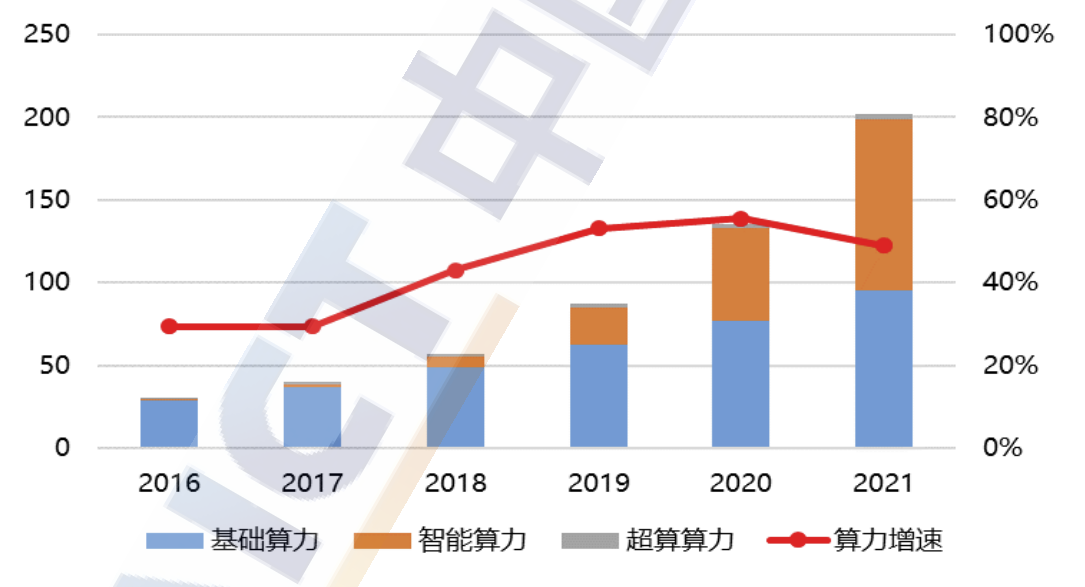
\includegraphics[width=8cm]{img/1.png}
	\bicaption{2022年中国算力发展状况\citep{china2022}}{China's computing power development status in 2022}
	\label{2022年中国算力发展状况}
\end{figure}

\section{计算机视觉算法工业化部署的特点与挑战}\label{计算机视觉算法工业化部署的特点与挑战}
\subsection{计算机视觉算法模型的生产过程}\label{计算机视觉算法模型的生产过程}
当前主流的计算机视觉算法,大多是基于监督学习的深度神经网络模型。通常,会使用标注过的图像数据集来训练算法,使其能在特定的业务场景下,可以输入数据中提取特征并做出正确的预测或分类。具体的,一个基本的模型开发过程,通常会先构造一个带有标注的基础数据集,并将其分为用于训练和调整模型参数的训练集(Train Set),用来验证模型精度和调整模型超参数验证集(Validation Set),和最终验证模型的泛化能力的测试集(Test Set)。模型经过反复调整后,当算法工程师在测试集上取得理想的结果,则模型生产的部分就基本结束。

\begin{figure}[htbp]
	\centering
	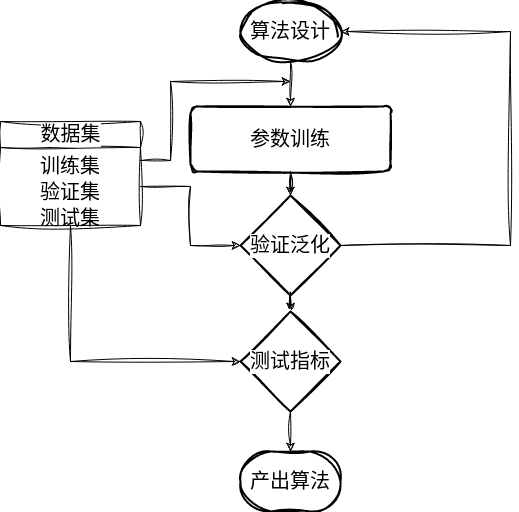
\includegraphics[width=8cm]{img/2.png}
	\bicaption{计算机视觉算法模型的生产过程}{The production process of computer vision algorithm model}
	\label{计算机视觉算法模型的生产过程}
\end{figure}

由于这一部分的工作主要在于网络结构的设计和参数的微调,而非具体的系统开发工程,因此通常选择更易用的python语言,并且基于api类似的几个通用框架(Keras、MXNet、PyTorch、Tensorflow、CoreML,etc)来实现,其生产的模型主要保证网络结构的准确描述,和对应参数的准确性即可,而不会过于具体的去优化模型推理的性能。其主要原因是考虑后续阶段,模型所需要部署的硬件条件和软件条件各有不同,有时还需要进行模型的精度压缩来获取更高的运行效率,由于深度学习模型大量依赖于矩阵计算,具有极高的并行性,因此非常依赖于计算机硬件层次的体系结构优化,在具体运行时环境不确定的阶段处理这一问题,不仅容易丧失软件的兼容性,同时优化效果也并不理想。

因此深度学习模型在部署前,还会再经历一段模型优化的过程,根据下游硬件的具体特性,对卷积一类的操作进行折叠和替换,以及对于整个计算过程的路径进行优化层间融合或张量融合(Layer and Tensor Fusion),常见的工具例如英伟达的TensorRT,Intel-cpu的OpenVINO,以及开源社区推动的TVM\cite{DBLP:journals/corr/abs-1802-04799},这些工具利用计算图和编译技术,通过算子融合,精度校准,计算时的内存分配等优化方式,提高了由基础训练框架直接生成的模型,在专有硬件上的计算延迟和设备的吞吐量, 例如TensorRT还针对动态尺寸输入进行了优化,pytorch直接生成的Torch Script模型\cite{paszke2019pytorch}在早期甚至没有这一功能。类似于开源社区的工具则具有更强的通用能力,通过编译技术,将神经网络模型所描述的计算图,表示为LLVM IR(Intermediate Representation),并利用包括机器学习技术参数搜索之类的方式进行自动优化,最终会根据后端的具体硬件(CPU,GPU,浏览器,FPGA等),自动替换为硬件级别深度优化的算子操作。

\begin{figure}[htbp]
	\centering
	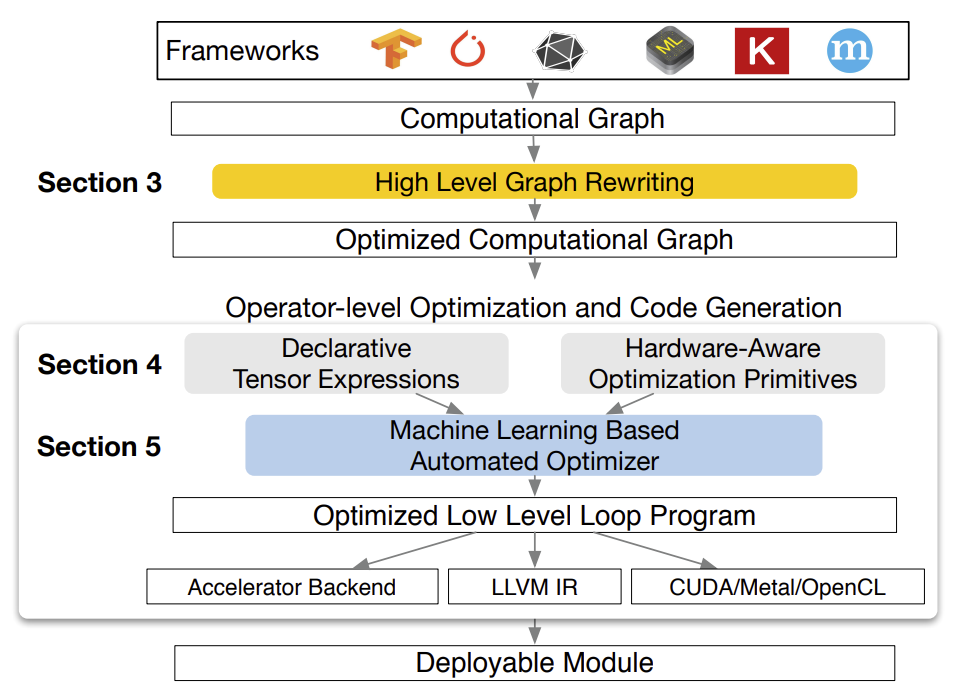
\includegraphics[width=8cm]{img/3.png}
	\bicaption{TVM架构图 \cite{DBLP:journals/corr/abs-1802-04799}}{System overview of TVM}
	\label{TVM架构图}
\end{figure}


\subsection{计算机视觉算法部署的实现与挑战}\label{计算机视觉算法部署的实现与挑战}
\subsubsection{传统视觉算法}\label{传统视觉算法}
传统计算机视觉的处理方法一般是多层次的,会通过多个层次的算子进行滤波和计算,获得不同的特征来做出决策。常见的包括颜色特征(颜色直方图),纹理特征(小波变换),形状特征(傅立叶形状描述符)等,基于不同的尺度,最知名的还包括尺度不变特征(Scale Invariant Feature Transform,SIFT\cite{ng2003sift})等,其作为重要的特征算子,和传统的机器学习算法例如支持向量机SVM(Support Vector Machine)和分类算法KNN(K-Nearest Neighbors Algorithm)结合使用,处理一些图像分类问题。这类算法对张量(Tensor)计算的专用硬件没有依赖,因此在系统角度而言,不涉及到硬件异构,所以产生的负载可以视为一般的CPU任务,在操作系统层面来进行处理和调度,仅需要描述好数据之间的传递和依赖关系。

\begin{figure}[htbp]
	\centering
	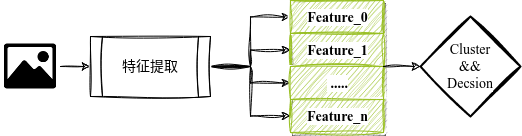
\includegraphics[width=8cm]{img/trad_vis.png}
	\bicaption{基于传统视觉算法的计算流程}{Computational flow of traditional vision algorithms}
	\label{基于传统视觉算法的计算流程}
\end{figure}

\subsubsection{推理部分}\label{推理部分}
当代深度学习算法,尤其是计算机视觉类算法,基本已经进化为一种端到端的模型(End-2-End), 不再需要手工设置特征提取和分类器等模块,以一整个深层模型,直接取代了传统算法的主体部分,并在分类,检测,分割,识别等任务一众任务中,精度指标相较传统算法取得显著优势。当前,工业领域应用最广泛的ResNet,YOLO,R-FCN等网络都体现出模型深层化的趋势,以Res-Net50\cite{he2016deep}为例,其网络包含49个卷积层和1个全连接层,其总体参数超过两千万,整体计算量超过38亿FLOPs,整个运算过程如果单纯的放置在CPU一侧,那么将就造成较大的计算延迟,无法满足实际业务场景的需求。

由于深度学习模型的推理和训练,其任务主要为密集的矩阵计算和梯度传播,重复度高,专用性强,且又因为应用广泛,具有较高的商业价值,因此厂商直接以ASIC(Application-specific integrated circuit)的形式,从底层硬件方面进行支持和优化的,推出了专门用于AI计算的半导体芯片。其内部的电路结构可以执行特殊的指令集,相对于普通的CPU,极大的增加了带宽和处理器的个数,同时将单个处理器的结构进行简化,在降低成本的同时,能快速执行简化后的指令集。其在运算效率和计算成本上,都和使用CPU相比有显著的优势。大多数情况下,视觉算法的模型推理部分,会尽可能的放置在针对矩阵计算和梯度传播有专用硬件模块的芯片(例如神经网络专用ASIC,GPU等)来运行,取得结果后再拷贝回CPU侧,调度原则相对不同于一般任务。

给部署阶段造成困难的还包括模型的持续迭代。计算机视觉算法是一个高速进步的领域,算法开发工程师经常需要推出新版本的模型。这种迭代一方面是来自于科学研究领域的不断进步,新的模型具有更高的准确率指标,或者是改进后只需要更少的参数,具有更优秀的推理延迟。另一方面则是由于视觉算法是基于有监督训练,其在上线的使用过程中,还会不断的收到来自用户或者自身团队提供的标注数据,这些数据会用于不断的扩充训练集,让模型具有更好的泛化能力和准确率表现。

虽然这一过程是在模型的生产环境完成,和部署过程属于独立的软件工程模块,按照开闭原则(Open-Closed Principle)仅需做到输入输出接口的一致性,即可让模型迭代和替换的过程独立。但实际的情况,新的模型在具体部署硬件上有支持差异。例如基于于注意力机制的Transformer\cite{vaswani2017attention}模型,由于其前后数据依赖程度远低于循环神经网络RNN和长短时记忆网络LSTM,大幅度改进的并行性能以及良好的表示学习能力,使得其在自然语言处理领域取得了巨大的成功,在机器翻译等任务中取得了非常优秀的表现,并拓展到视觉领域,例如ViT(Vision Transformer)\cite{khan2022transformers}。

虽然在训练侧得到实现,但部署方面,很长一段时间仅有官方训练框架直接生成的模型可用(例如pytorch直接生产的TorchScript模型),缺乏对硬件支持优化。即便是生态最完善的英伟达,也花费了接近3年(2017年发表,2020年3月发布TensorRT7.2)才支持将常见的Transformer模型(BERT、GPT-2等)转换为TensorRT\cite{tensorrt7}可识别的格式。与此形成对比,华为直到昇腾AI异构计算架构CANN 6.0(2022年11月发布)\cite{HuaweiCANN},才首次支持\verb|torch.nn|的Transformer Layers算子。

无论是出于实际的经济成本,还是整个智能化软硬件的国产可控,目前有相当大比例的客户,在软件的集成采购中,会要求使用指定的品牌范围的硬件设备。这导致在推理部分的实现上,更具体的描述是,一个服务于相同请求的计算机视觉算法服务系统,可能同时使用多种不同的模型,运行在多种不同的硬件环境上。因而需要充分考虑到不同硬件之间混合部署和模型替换需求,做好硬件负载和推理延迟的评估,防止使用参数量不同的模型,尽量协调整个计算流水线的吞吐执行。

\subsubsection{前,后处理部分}\label{前,后处理部分}
工业化算法的部署场景需要更多的处理步骤,例如最常见的输入摄像头输入,传入图像往往有不同的尺寸和清晰度,除了传输过程中的压缩和解编码,还包括一些根据后续算法定制化的额外操作。一个常见的例子是,经常作为提取特征的卷积神经网络ResNet,其输入需要大小为固定的$224\times224$,像素值经标准处理后在$[0, 1]$或$[-1, 1]$范围内的浮点数矩阵,因此输入之前需要使用填充(Padding)的方式,将输入图片缩放至一定尺寸,再将其嵌入到一个大的黑色图像中,使其能够适应ResNet的输入,或者也可以通过裁剪(Cropping)将输入图片从中心裁剪为固定比例。这部分的计算称为数据的前处理(preprocessing),属于端到端模型以外的范畴,对应在输入图像经过神经网络模型之前对其进行的一系列操作。

常见前处理包含:
\begin{itemize}
	\item[$\bullet$]尺寸缩放(Resize):将输入图像调整为神经网络模型指定的大小,避免图像大小的差异对模型性能的影响。
	\item[$\bullet$]归一化(Normalize):将图像像素值缩放到固定的范围内,如$[0,1]$或$[-1,1]$,有利于提高模型的训练速度和准确度。
	\item[$\bullet$]色彩空间类型转换(Color space type conversion):将图像从RGB(Red,Green,Blue)色彩空间转换为其他色彩空间,如灰度图像或HSV(Hue Saturation Value)色彩空间,可以更好地提取图像的特征。
	\item[$\bullet$]解码(Decode):对于一些视频和图像数据数据,传输的过程可能会按照一定的编码方式进行压缩,需要解码之后在进行处理。
\end{itemize}
和前处理形成对应,计算机视觉算法同样包含后处理过程,后处理(postprocess)通常是指对算法输出的结果进行一些加工和过滤,以得到更加准确和可靠的结果,相对前处理而言,后处理逻辑相对会更复杂。常见的后处理包括非极大值抑制(Non-maximum Suppression,NMS)\cite{bodla2017soft}、去重、后验概率校准等。例如,在目标检测算法中,算法输出的是一组候选框(Bounding Boxes),需要经过NMS算法去除高度重叠的框,并进行类别预测和后验概率校准,最终得到检测结果。人脸识别算法中,通常会对算法输出的人脸特征进行去重和归一化,以提高识别准确率。后处理的目的是提高算法的准确率、鲁棒性和速度,并适应不同的应用场景。

前,后处理是计算机视觉算法中非常重要的环节,可以极大地影响模型的性能和准确度。然而不同的算法需要进行不同的前,后处理操作,其实现方式非常多样化,常见的原因包括:
\paragraph{专用硬件支持}虽然前处理和后处理的运算并非完全如推理模型一样,表现为纯粹的张量运算,但其仍然会包含很多显著的并行优化点,其原因主要在于图像信号本身就被表示成矩阵形式,其处理天然符合一些线性代数的运算优化方法。现代图形芯片出于渲染管线(Render Pipeline)高并行度的计算任务需求,设计了大量的流处理器和高带宽,被逐渐拓展运用在一部分类似的通用计算环境。因此例如经典的图像处理库OpenCV\cite{bradski2000opencv},早在2010年就开始着手将传统图像处理的部分算法,包括常用的前处理和后处理,利用NVIDIA的CUDA\cite{sanders2010cuda}编程模型来实现。

长期以来,国内的计算芯片发展,一直面临如X86指令集这类的专利授权问题。ASIC芯片因为不需要考虑固有的软件生态,因此相对容易回避限制,被广泛视为产业自主化的机会之一。经过数年的发展,有类似于华为海思这样的借助旧有芯片设计业务的入局者,也包括寒武纪,壁仞这类专精于此类芯片的创业公司,其整体呈现出较强的多样化趋势。相较于训练框架逐渐因为软件生态逐渐走向统一,专用的计算芯片没有兼容性的考虑,不同于GPU通常采用IEEE 754标准的浮点数运算,ASIC芯片以更强的专用性目的而实现,采用定点数运算、半精度浮点数运算或其他非标准来适应训练或者部署的场景,只需要能正确的执行模型,输出精度差距保持在一定范围内即可。

然而由于ASIC芯片设计的定制性太强,因此为了保证主要场景下的性能和效率,有时会限制芯片在其他任务上的可用性,难以像CUDA一样抽象出一套完整的并行计算框架。同样也因为开发时间较短的原因,软件生态和NVIDIA相比还有难以逾越的差距。前文所提到推理加速器TensorRT,支持以插件的形式,增加框架训练输出模型以外的额外部分,包括例如\verb|leaky relu|\cite{xu2015empirical}这样的网络层, 还可以以类似的形式将一部分前处理和后处理操作,封装到推理模型内部,得到通用优化,CUDA也可以直接编写运行在GPU上的并行程序,进行灵活的显存管理。

\begin{figure}[htbp]
	\centering
	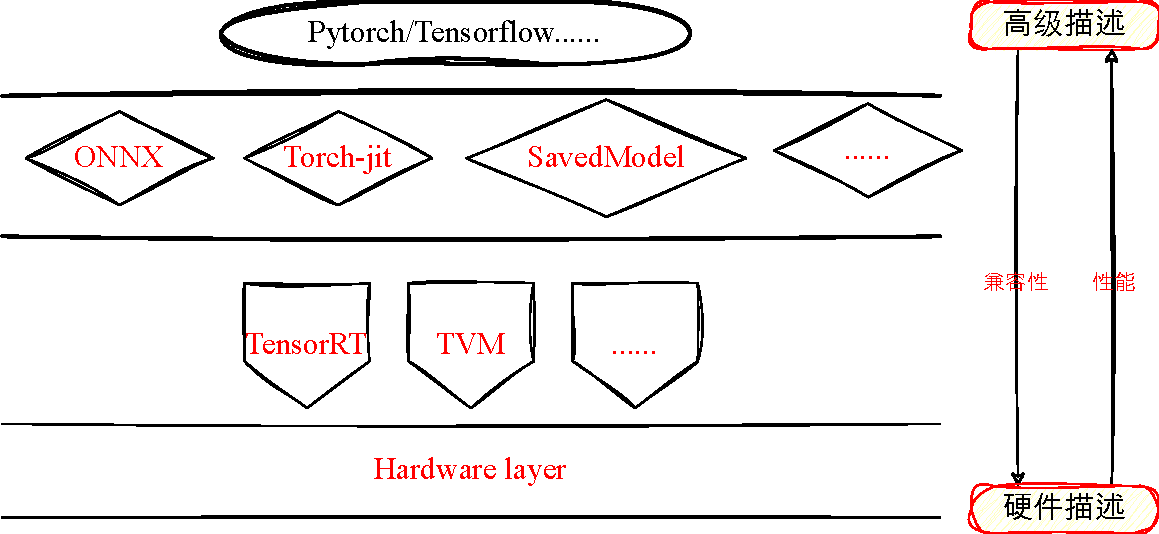
\includegraphics[width=8cm]{img/4.pdf}
	\bicaption{视觉算法模型的兼容性和性能权衡}{Compatibility and performance trade-off of vision algorithm model}
	\label{视觉算法模型的兼容性和性能权衡}
\end{figure}

而国内硬件设备在软件的完善程度参差不齐。一个具体的例子是,作者于2022年初进行华为ASCEND加速卡相关开发过程中,发现其专用的达芬奇计算卡更多是支持通过API的方式去调用一些固定算子,定制化的函数仅可通过组合实现,缺乏更加底层的接口,由此导致部分前处理,后处理的代码不能支持,仅能放置在CPU侧来运行,进而引发数据在ASIC芯片显存和通用内存之间来回拷贝的额外的开销,需要重新考虑调度安排。
\begin{figure}[htbp]
	\centering
	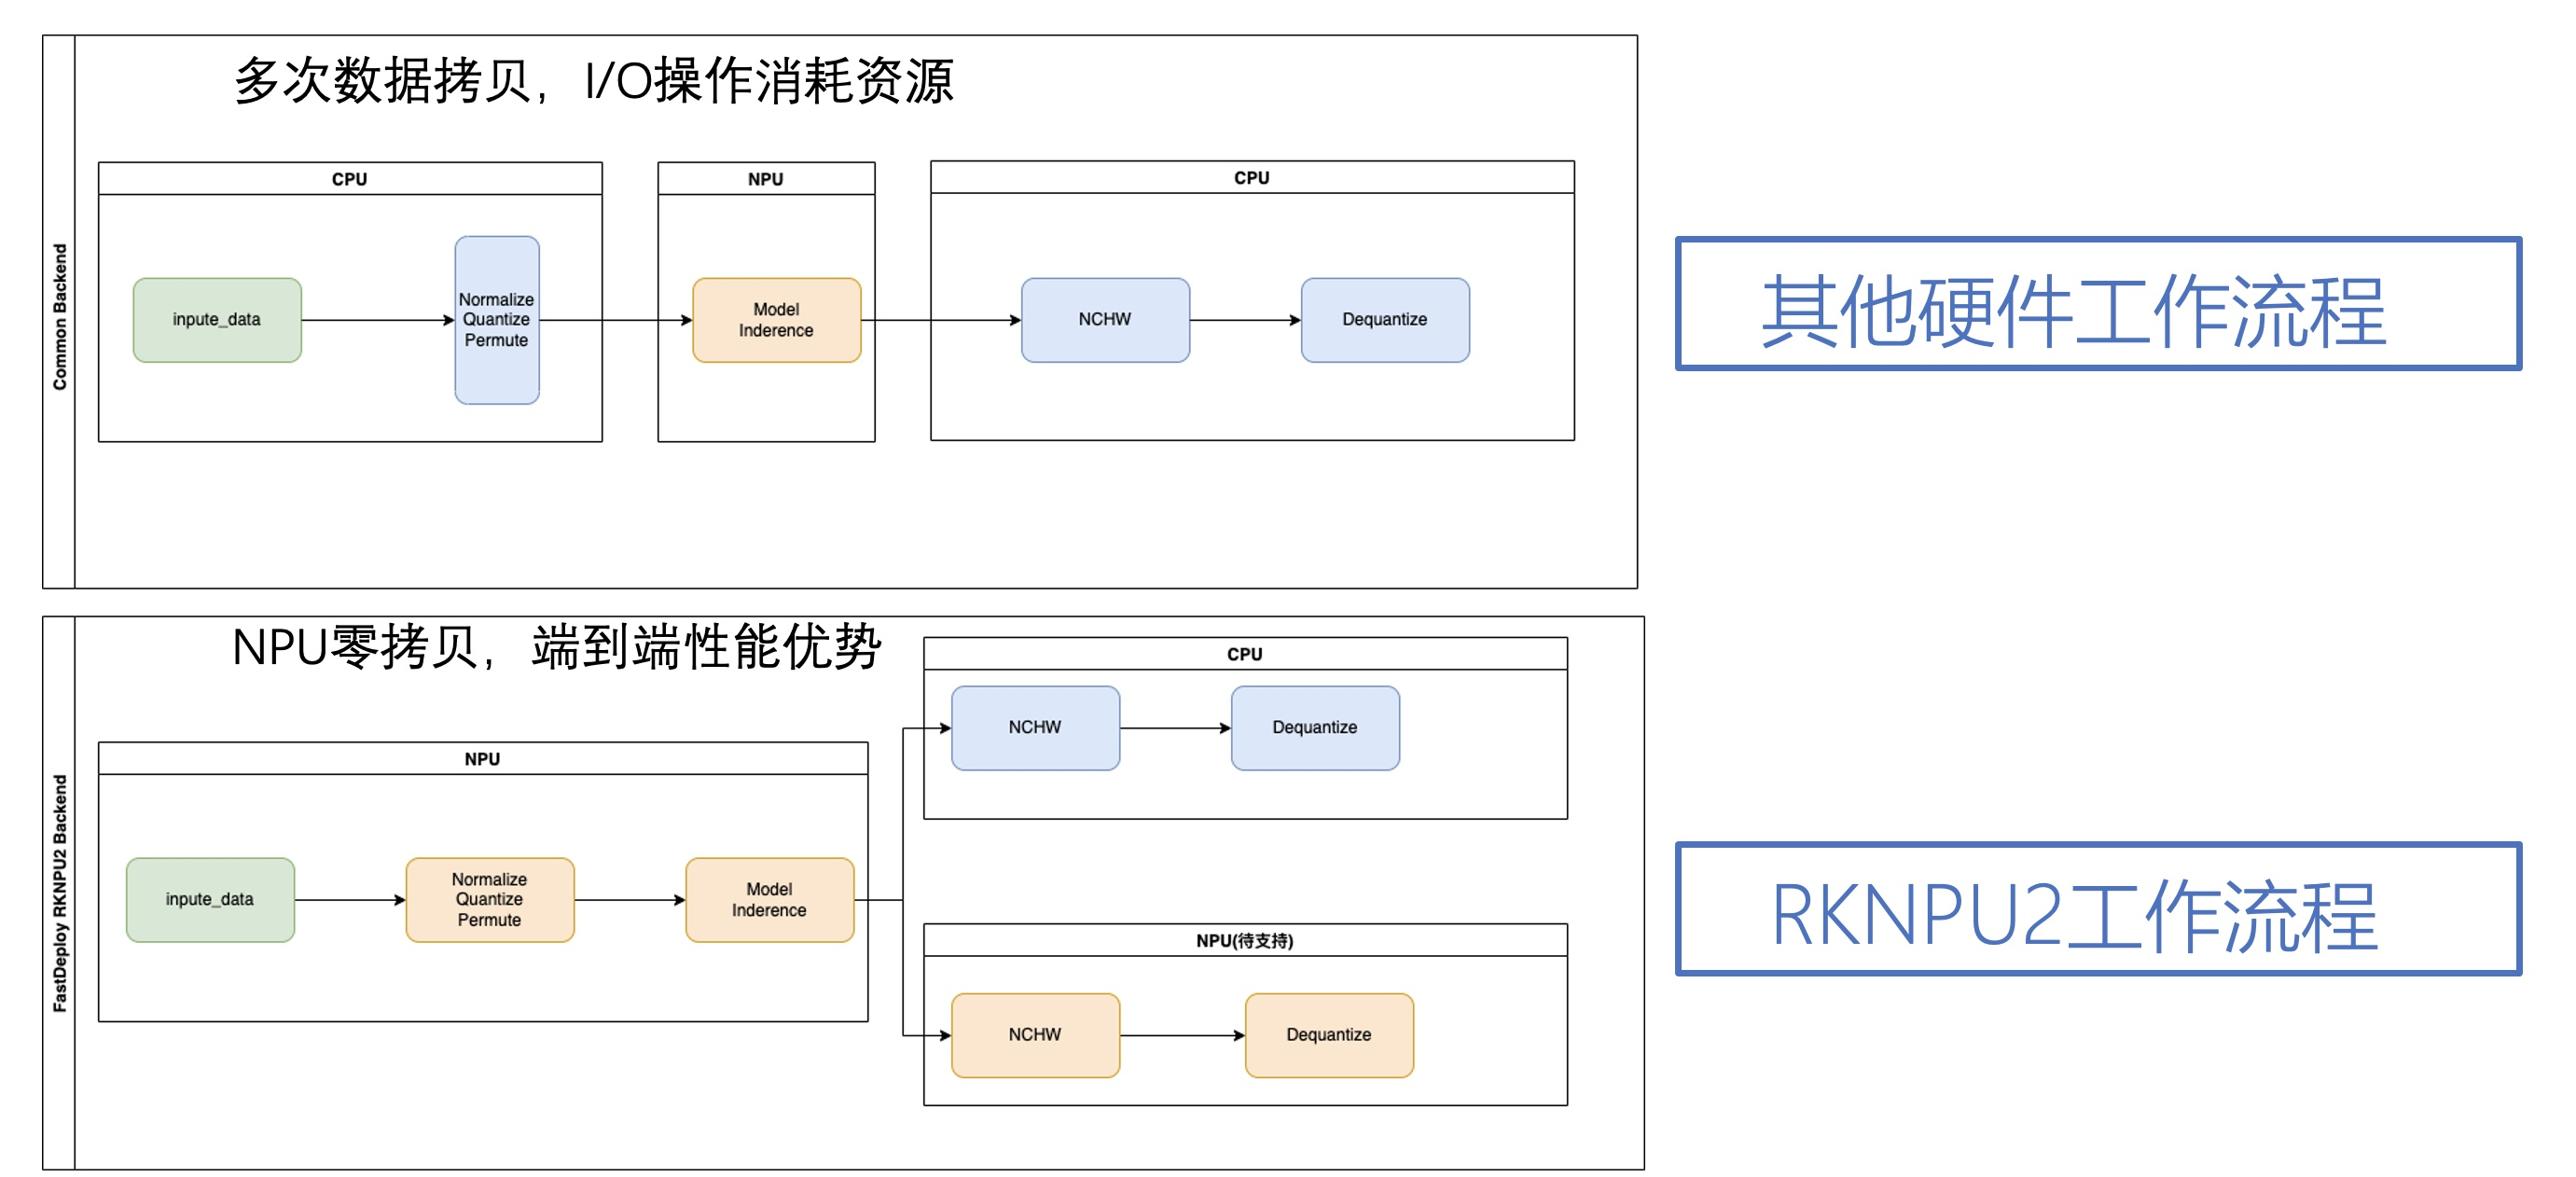
\includegraphics[width=8cm]{img/rknn_support.jpeg}
	\bicaption{rk芯片集成处理(目前暂无)\cite{rknnprocess}}{rk chip integrated processing(still not support)}
	\label{rknn-support}
\end{figure}

上述讨论说明,由于部署阶段既要贴近硬件的性能优化,又要满足多种硬件的适配,因此必然导致高度的软件封装,同一函数接口的执行开销难以评估,进一步影响到软件层面的实现和调度。
\paragraph{计算成本和开发难度}
相较于Intel最新的桌面级CPU-13900k,即便考虑AVX(Advanced Vector Extensions)512指令集的SIMD(Single Instruction Multiple Data)和FMA(Fused Multiply Add),其理论算力约为RTX4090的3$\%$($\geq$100TFLOPs),仅考虑单位算力成本,尽可能的去选择GPU是一个更合理的选择。然而在实际的应用场景中,CPU的主要功能远不止完成计算,而是执行更加多样性的活动,例如需要频繁中断的网络和IO(Input/Output)业务,常需要配置多核心来提高响应速度,主频则少有满载的情况,甚至普遍不足峰值10$\%$, 生产实践中遇到的情况是,负载最高的硬件往往是专用的深度学习计算卡,CPU的反而不是性能的瓶颈所在,计算资源常有冗余。一般情况下,部署原则是尽可能使GPU,ASIC部分硬件达到最高的利用率,部分前处理,后处理的是否放置在GPU等设备上执行并不固定。

除去硬件考量,即便是有完善文档和调试工具链的CUDA,编写面向GPU的并行程序也对体系结构知识有一定门槛,软件工程师的开发难度同样需要考虑。一般的,对于不构成性能瓶颈,在总体延迟中占比较低的处理,会直接选择以CPU侧实现来节约开发人员的时间,对于通用性高,时间开销大的算子,会考虑针对具体的硬件去做特化的实现,以此来降低开发人员的实现难度,便于合作的和迅捷开发。

\subsection{计算机视觉算法模型的部署外环境}\label{计算机视觉算法模型的部署外环境}
上述过程讨论了计算机视觉算法,在计算层面将整个推理过程进行包装,对外提供稳定的抽象功能接口(动态库,远程过程调用(Remote Procedure Call,RPC)),内部完成模型的加载和版本管理,并对不同的硬件支持进行实现过程,这种方式可以近似的表示为下图:

\begin{figure}[htbp]
	\centering
	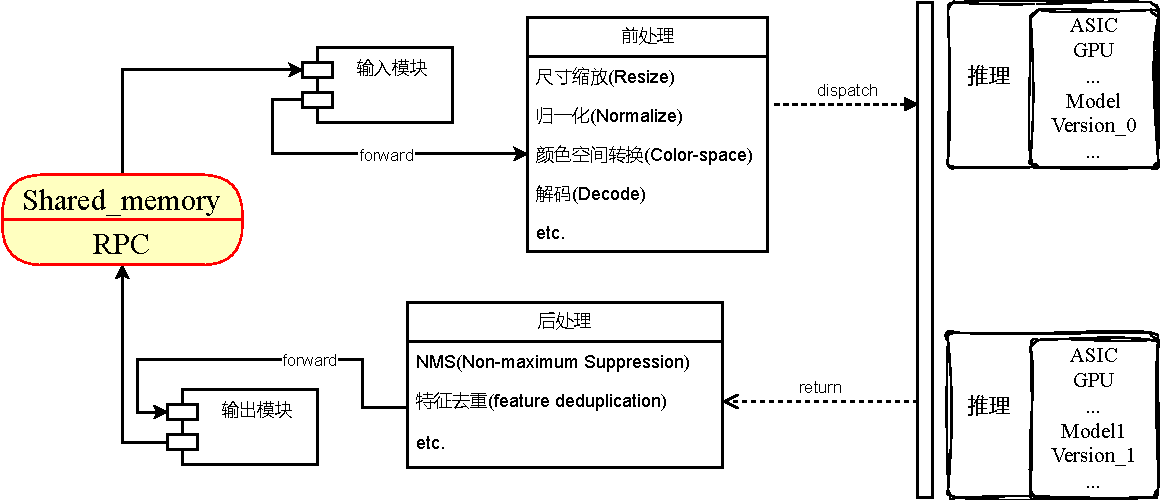
\includegraphics[width=8cm]{img/frame.pdf}
	\bicaption{计算机视觉算法部署框架}{Computer Vision Algorithm Deployment Framework}
	\label{计算机视觉算法部署框架}
\end{figure}

我们在此定义部署的外环境,指包含从数据输入到结果输出,各个环节的运行环节。即我们将整个推理侧视为一个完整的服务端来考察,如\ref{计算机视觉算法部署框架}所示,其部署的外环境包括软件本身的运行环境,以及数据的传输交互(输入输出模块)。

对基于深度学习的算法而言,一个成熟的落地场景是推荐系统,例如网络购物平台的商品推荐,或者内容平台的视频和文本推送。这一类型业务的特点是数据和计算硬件物理空间相近,处于同一数据中心,通常还有专用的传输线路。同时,对延迟的稳定性要求不高,更强调单位计算的成本更低和高并发下的可拓展性,外环境基本近似为基于虚拟化技术云计算平台。

实际场景中视觉算法更偏向于现场部署,用户基于成本考量,以及数据的安全问题,并不希望使用云服务。举例一个港口项目的情况,内部系统集成了集装箱破损检测,区域门禁,人员安全帽行为检测等多样化的业务。虽然需求多样,但并发量小,处理的数据量规模低,大部分时间只执行有限种类的目标检测,出现需要进一步识别的概率不高。这种部署,区域内一般有中心化的机房,数据的传输经由内网,通常会集中式的混合部署一些服务,比如简单的Web程序和数据库等。

一种更为广泛的情况则是基于边缘计算的部署,其主要目的是通过在用户或数据源的物理位置附近进行的计算,以此降低延迟,节省带宽。工业场景下的分类和检测,当任务相对复杂时,除去算法的实际功能指标外(Recall/Precision),通常还会对服务的质量提出较高的要求,例如可靠性和延迟响应速度。这种情况多见于安防和政府治理等领域,虽然其主观目的是提供可靠易用的智能化服务,但同时也必须考虑到数据安全和隐私保护的问题,因此一般不会长时间保存待分析数据。同样,嵌入式系统下硬件资源无法进行弹性拓展,使用缓存队列一类的组件保存待处理请求,需要控制在尽量小的规模以防止过度占用内存。

由于请求基于流式(Streaming)\cite{muthukrishnan2005data}处理和输出,这类系统并非完全强调实时性(Real-time),而是允许请求在一个小的窗口期内完成,即信息的输入,检测结果的输出之间可以有一段的窗口延迟。举例说明,跟踪高速行驶的车辆,并对其属性信息和特征(车辆的颜色,类型), 车牌号码等做出识别,同时甄别是否有违章行为,这个过程允许有一定的延迟,但会非常强调延迟的稳定性,因为流式处理下,请求积压后只能丢弃数据,可能导致应被监测的非法行为遗漏,以及统计信息丢失。

\begin{figure}[htbp]
	\centering
	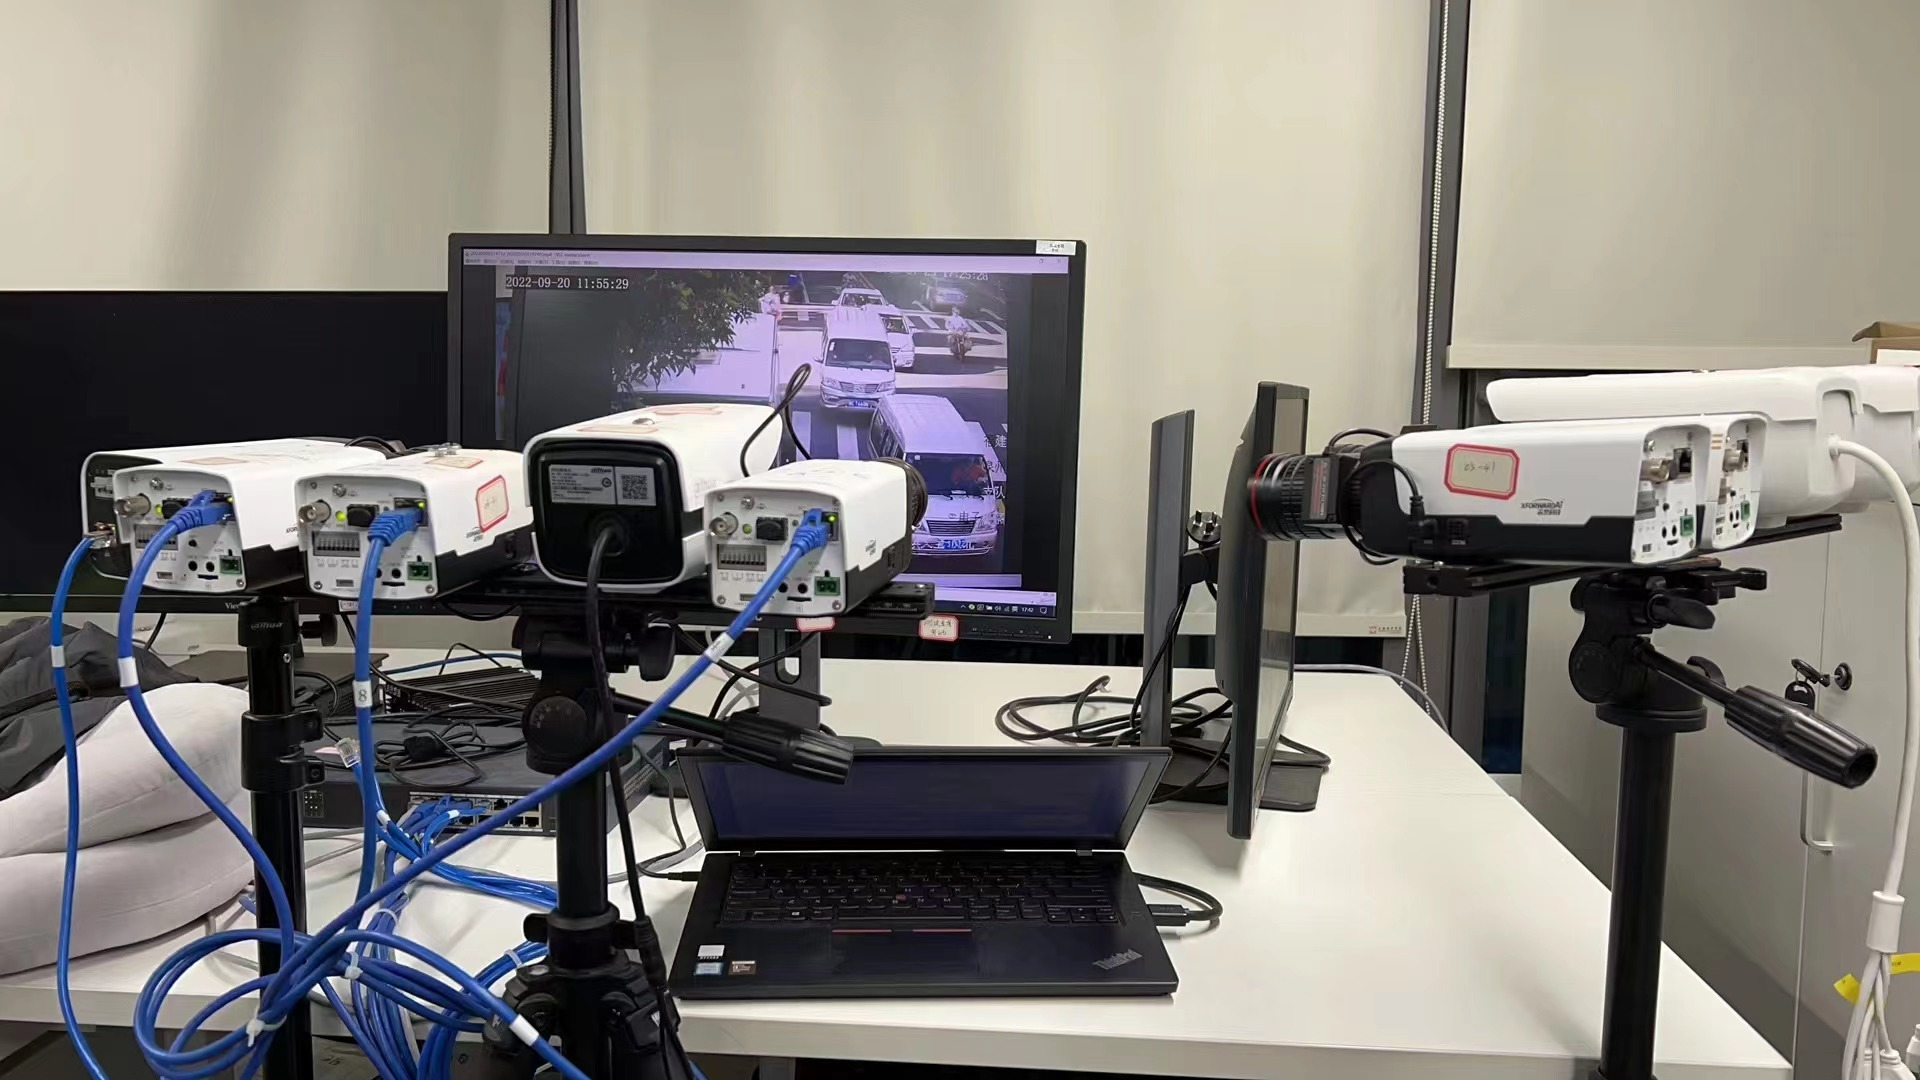
\includegraphics[width=8cm]{img/hd.jpeg}
	\bicaption{有线直连的超清摄像头(拍摄于实习公司)}{Ultra-clear camera with direct cable connection (taken in my intern company)}
	\label{有线直连的超清摄像头}
\end{figure}


如图近似描述了类似的架构场景,摄像头配置在道路的不同的位置,信号清晰度普通的低功耗摄像头,会被安装在交通信号的灯柱上,通过WIFI将数据传输到本地的路由器,或者直接通过5G移动网络。而部分体积大,功耗高的高清晰摄像头,则会链接到专用电源,通过有线网络的形式传输到本地的路由器。路由器再将数据传输到边缘设备,多路聚合的视频信息会通过计算机视觉算法进行处理和计算,运行车辆,驾驶员的属性检测和行为识别算法,最终将获取的信息传入防火墙以外的数据中心,进行存储和进一步的额外服务。

\begin{figure}[htbp]
	\centering
	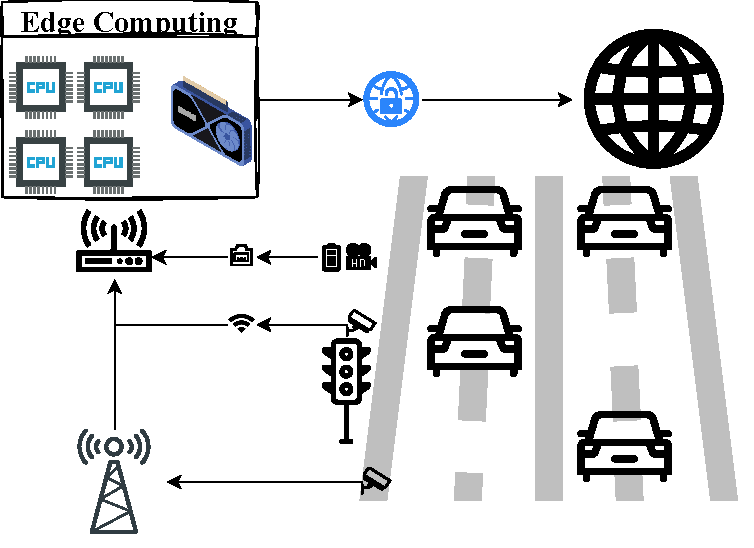
\includegraphics[width=10cm]{img/trafic.pdf}
	\bicaption{交通场景的边缘计算部署}{Edge Computing Deployment in Traffic Scenarios}
	\label{交通场景的边缘计算部署}
\end{figure}

参考上述示意图,不难发现,以边缘计算形式对计算机视觉算法进行部署,其整个运行的流程除去\ref{推理部分}描述的推理部分和\ref{前,后处理部分}的前,后处理以外,其整体延迟和可靠性还和传感器到运算部分的传输过程有关。例如,无线网络传输的延迟,会因为传输距离,信号干扰,障碍物等原因增加,移动网络则更容易因为用户数量过多而导致网络拥塞,同时,因为帧率和分辨率的不同,各个图像传感器自身也因为传输数据量也不同。即便我们考虑推理过程的封装,将其视为绝对可靠,但由于计算机视觉算法的部署外环境的特点,无法像虚拟化平台一样提供容错和备份性能,边缘计算硬件,网络,接口在内的设备任一节点故障,都将影响整体服务质量。区别于传统的虚拟化服务器,出于数据安全和隐私保护,局域网和边缘计算的场景,导致我们难以获取足够的信息,传统的运维工具难以对故障进行快速的定位和考察。

\section{计算机算法延迟监测的意义}\label{计算机算法延迟监测的意义}
从算法工程师所完成参数调试的模型,到具体部署为平稳运行的推理服务,不仅需要具体考虑软件,硬件的兼容性和复杂性,同时还涉及到工程成本,以及部署外环境的稳定性问题。了解各个步骤运行时间在整体运行过程中的占比,不仅可以在计算过程中作为优化指引,满足性能调试方面的需求。同时,面向一些对于延迟可靠性要求较高的,以流式视频输入的分类检测任务,我们同样也需要一些传输延迟方面的信息,对\ref{计算机视觉算法模型的部署外环境}里提及的外部部署环境故障进行事后跟踪和故障定位。

对于一般端对端的服务请求,会使用QOS(Quality of Service)来进行衡量。传统意义上这一指标主要用于计算机网络中具有实时需求的业务。其用于评估任务是否能够以可接受的延迟,稳定响应请求的发起端,例如对于语音通信,视屏会议等应用场景,需要准确,快速的在服务端和客户端之间传递数据信息,以达到较好的信息交互体验。QOS的作用即为评估例如网络延迟,丢包具体会对服务的质量造成多大的影像,具体的,例如会对信息的完整度,卡顿,清晰度等进行量化的评估,进而作为应用程序在带宽分配,传输调度上的参考,以满足用户的需求。

计算机视觉系统的部署一般分为内部调试和外部发布两个开发阶段,内部调试主要以正确性验证为主,容许较为宽松的额外负荷,对外发布阶段则需要考虑性能,功耗等多方面的问题,对视觉算法这类延迟和资源受限的应用,尤其是部署在边缘计算硬件的情况下,还需要考虑系统运行具体环境,调整一些参数设置。由于正确性依赖于模型算法本身,因此如果想评估视觉算法的QOS,作为优化方面的参考,应当用响应时间,即延迟方面来进行衡量。

此外,对于部署的外环境下故障难以定位的问题,延迟的记录可以对计算机视觉算法的部署平台,给出一定的事后追踪能力。主要方法为在视觉算法运行过程中记录和延迟相关的日志,当出现故障或错误时,通过查看延迟及其相关的元信息来追踪故障的发生位置,有助于更好地了解系统的运行情况和发生的事件,提高系统可观测性与可靠性。

\section{现有计算机视觉算法延迟观测的一般方法与不足}\label{现有计算机视觉算法延迟观测的一般方法与不足}
对计算机视觉算法的延迟观测,至少应包含以下几个步骤:
\begin{itemize}
	\item[1]在算法的关键阶段(如网络传输,文件系统操作的IO事件,图像前,后处理,特征提取、分类、检测推理等)插入日志记录代码,记录节点时间戳和一些程序上下文。
	\item[2]计算每个阶段的耗时,可以通过将结束时间减去开始时间来计算每个阶段的耗时。这些耗时信息可以记录在日志文件中,也可以通过其他方式进行收集和处理。
	\item[3] 将收集到的延迟信息进行可视化和分析,或者输入算法获取一些指标作为评估参考。
\end{itemize}
从实现的角度,除去多样化的指标分析环节,可以将上述过程分为事件观测和日志记录两个阶段。

\subsection{延迟事件观测}\label{延迟事件观测}
传统的延迟事件观测,主要有硬件工具和代码注入日志两种方式

\paragraph{基于硬件支持的性能分析(Profiling)工具}

出于性能调试和观测的目的,硬件厂商会提供一些专用工具,来分析算法时延。例如Nvdia的Nsight Compute\cite{yang2020hierarchical}就是其中一种,通过CUPTI(CUDA Profiling Tools Interface)进行收集,利用可视化工具提供一个相对直观的界面呈现结果。

\begin{figure}[htbp]
	\centering
	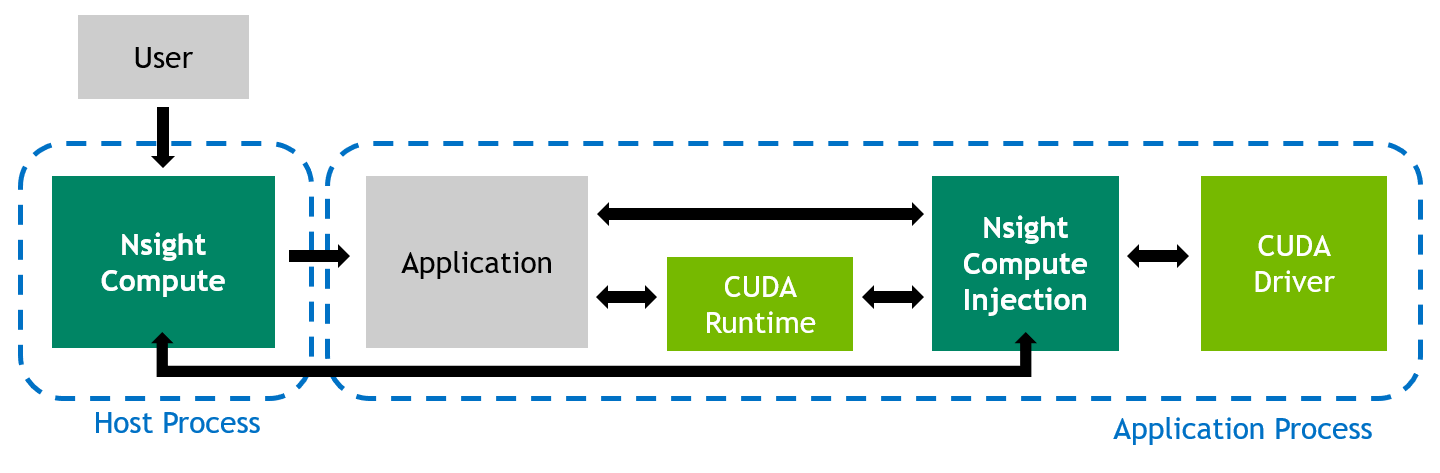
\includegraphics[width=8cm]{img/nsight.png}
	\bicaption{Nsight Compute的观测原理}{Observation principle of Nsight Compute}
	\label{NsightCompute的观测原理}
\end{figure}


这一做法的主要缺陷在于兼容性和局限性。兼容性主要体现在这一方法依赖于硬件厂商的软件支持,不适合需要部署国产ASIC芯片设备的混合部署场景。局限性体现在,工具对于性能观测的颗粒度缺乏定制性,对于运行阶段的时间划分是直接通过函数为单位,缺乏可定制性,更适合开发者来使用在发布前的调试分析阶段,查找整体的计算负载瓶颈。另外因为其捕获的信息颗粒度深入到指令集的层面,并且依赖于一套较为沉重的图形界面(Graphical User Interface,GUI)工具,以嵌入式实时观测的角度来说,还存在性能负担过于严重的问题,一般更适合在云服务端的部署上使用。

\paragraph{基于代码注入的日志记录}
更加轻量级的做法,是在软件代码中嵌入日志记录程序,以字符串的形式记录时间和延迟情况,例如使用std::chrono库等C++时间函数,或使用Python中的time.time()等函数,同时也可以定制化的去获取一些程序的元信息(例如上述CUDA Profiling API或者其他),例如:
\begin{lstlisting}
#include <cuda_runtime_api.h>
int device_id = 0;
cudaDeviceProp prop;
cudaGetDeviceProperties(&prop, device_id);
int gpu_utilization, memory_utilization;
cudaDeviceGetUtilizationRates(&gpu_utilization,\
&memory_utilization);
\end{lstlisting}
使用这种方式来记录延迟信息的一个问题是性能,作为一个运行时的延迟观测装置,我们希望记录时间的代价尽可能的低,而无论哪一种程序的时间函数,都依赖于操作系统的系统调用。大多数情况下,日志信息还需要保留一些额外的元信息(Meta Data),例如CPU和GPU(ASIC)的运行时状态,以及内存占用,进程参数堆栈等用于事后追踪时故障定位。这将反复进行程序上下文切换(Context Switch),和从内核态(Kernel Space)读取到用户态(User Space)的复制。同时,在用户态生成字符串日志,需要首先需要通过参数填充(Parameter Handling),再从保存的数据中生成文本(Text Processing),这些都会引入一些在嵌入式环境下不容忽视的性能开销,应尽量优化和避免。另一不足是这种日志生成方式,任何对日志产生过程的修改,都必须重新编译整个软件,维护难度较大,导致观测延迟为目的注入部分与本身的业务代码深度耦合,在软件工程的角度并不合理。

\subsection{延迟日志记录}\label{延迟日志记录}
延迟信息及其附属的元数据作为日志的形式写入,可能因为IO问题干扰正常的操作系统调度,因此将日志进程和软件任务本身分离,以提交(Commit)的方式,让日志进程独立完成记录持久化(Persistence),是一种常用的优化思路。在边缘计算的场景中,一个典型的设计就是基于发布-订阅模式(Publishers + Subscriber),即软件工程中的观测者模式(Observer Pattern),通过集中式的提交,构建专门的日志系统,还可以用来辅助调度功能。其所有的提交均通过基于网络的RPC接口,类似的框架包括Kafka\cite{kreps2011kafka}、RabbitMQ。 Kafka 专为高吞吐量而设计,而RabbitMQ允许发布者和订阅者之间的复杂路由\cite{dobbelaere2017kafka}。


边缘计算设备,或是服务器中,以进程为单位运行的计算机视觉算法实例,作为日志发布者(Publishers),统一向日志进程订阅者(Subscribers)提交产生的日志事件信息。这种模式的优越性在于具有很强的解耦性,边缘设备和独立运行的计算机视觉算法实例,启动后可以随时注册到日志进程中,只需确定好提交的方式,无需对日志系统进行修改,各自独立地进行操作,同时系统可以采用分布式消息队列等方式来保证日志信息的可靠性,避免信息丢失或重复传递等问题。订阅者通过处理和分析日志信息,帮助管理者监控和调试边缘设备和系统的运行状态,以此提高边缘计算的可靠性和稳定性。但缺点也非常显著,即网络消息传递的开销增加了带宽压力,并且中心的调度和日志接收节点需要显式的管理,造成了一定的运维难度,在部分性能要求较高的场景下,
框架仍然显得过于沉重。

\begin{figure}[htbp]
	\centering
	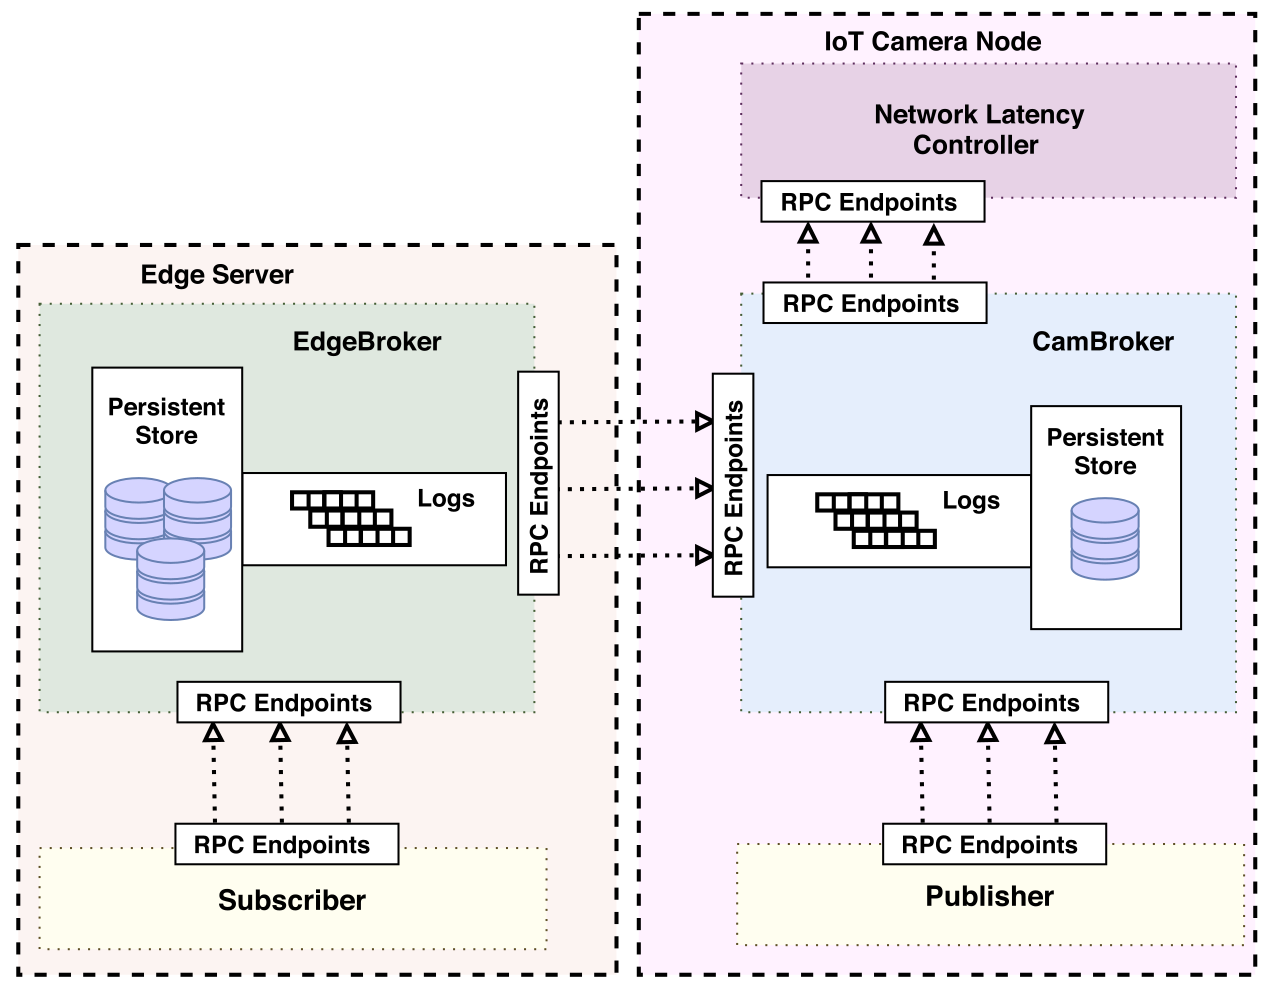
\includegraphics[width=8cm]{img/rpc_log.png}
	\bicaption{基于发布订阅的边缘计算日志系统\cite{george2021mez}}{Edge computing log system based on publishers + subscriber}
	\label{基于发布订阅的边缘计算日志系统}
\end{figure}

另外,日志写入无论是集中式还是独立进行,写入文件或发送到远程服务器的操作都无法避免,尤其是在IO速度较慢的嵌入式系统中,可能会导致系统的响应速度变慢。一些日志系统支持通过日志级别过滤的方式,只记录重要的日志信息,并采用缓存机制,批量记录日志信息,减少IO操作次数,提高系统的IO效率。也包括使用异步处理,避免IO操作阻塞主线程或进程的执行。但在嵌入式系统中这类资源受限的环境下,实现以上操作时,还需要关注减少软件依赖,以及日志信息的细节问题,各个环节的衔接问题,往往需要定制化的落地方案。

\section{论文研究内容和创新点}\label{论文研究内容和创新点}
\subsection{论文研究的出发点}\label{论文研究的出发点}
本文研究源自公司业务实践中的需求,也来自开源社区的启发。在计算机视觉算法落地部署的开发过程中,由于公安政府,工厂等客户需求各有侧重,并且需要同时针对寒武纪,华为,英伟达等不同的底层硬件,抽象出统一的接口,进行兼容和封装测试,以网络服务或者静态库依赖的方式,提供给更上层的业务框架来进行调用。因此经常需要进行各类不同目的的优化,甚至有时优化的主要目标是节约异构部分的硬件成本(减少ASIC和GPU的用量),这在传统信息服务中是不可想象的。

在这一过程中,延迟数据作为一个重要的优化参考,需要在每次测试中反复采集。基于传统方式的延迟事件观测,体现出了较大的局限性,在观测能力,观测维度,观测灵活性等各方面均有显著不足,且日志格式不统一,难以进行可视化。在此过程中,意识到SDK(Software Development Kit)独立可观测模块的缺乏,于是开始着手实现相关功能。

考虑到实际项目中,经常发生维护工程师远赴现场,结果只是简单的接口故障或者网络问题。因此也希望这种可观测性能满足一些边缘计算"盒子"在使用过程中的故障定位和事后追踪能力。

在对开源社区寻求解决参考的过程中,发现单纯引入一个更高性能的日志记录器,并无法解决部署环节复杂的延迟观测需求。而一种应用在无人驾驶领域,基于动态观测技术的定制化方法\cite{bpfgpu}则给予了思路启发,由此实现了一个基于内核BPF(Berkeley Packet Filter)\cite{mccanne1993bsd},和业务系统深度融合的轻量延迟观测系统。
\subsection{论文的主要内容}\label{论文的主要内容}
论文聚焦于计算机视觉算法延迟观测这一具体需求,具体讨论了如何在部署流程相对成熟的,2D识别,检测,分割这类业务时,面对复杂的部署条件,尤其是在边缘计算的场景下,如何以较低的代价,获取数据在各个环节的执行延迟,并拓展观测到一些常规运维工具无法获得,或者获取成本较高的底层状态数据。同时,也考虑到了这些数据在嵌入式系统中,如何在尽可能不影响业务代码运行的情况下,以尽可能低的代价得到保存。

论文的主要内容即探讨了这一轻量延迟观测系统的技术选型和实现细节,基于绝大多数视觉算法部署,都会运行在Linux系统的客观事实,论文的设计以放弃对早期操作系统版本的兼容为代价,全面采用Kernel5.8(发布于2020年)\cite{bpfring}之后的新特性,换取了适合嵌入式系统的低依赖和高性能。通过将BPF的用户态插桩技术,运用到计算机视觉算法模块化封装的实现中,借助对操作系统动态观测能力的二次开发,极大拓展了SDK的观测自由度,大幅度降低了延迟观测所需的工作量,并给出了面对不同硬件,不同的软件支持方式下,如何处理兼容问题的解决参考。

同时,通过实现一个延迟信息专用的,独立的轻量级日志系统,进一步完善了整个工具的可用性。此处充分利用了内核原生异步IO(Io- uring)\cite{axboe2019efficient}新特性来提高性能。同时充分考虑了延迟信息的具体特点,通过设计定制化的存储格式,引入前置过滤的运行时算法,实现了对延迟记录过程中的性能优化,也让数据更便于后续的分析和使用。

进一步的,论文通过设计仿真实验,讨论了这一观测系统所捕获的持久化日志,如何在计算机视觉算法任务场景中得到应用。通过对基于计算图的计算机视觉算法部署方式进行模拟,在最新的国产ASIC芯片上实践了包括如何利用延迟数据,作为部署优化的参考信息,以及故障后,如何利用延迟数据进行简单事后追踪的问题给出了简单的测试。

\subsection{论文的创新点}\label{论文的创新点}
论文的主要创新点在于,给出了在基于计算图-模块封装的计算机视觉算法部署框架下,如何引入内核动态观测的实现方案,并从原理上对性能优化和功能实现进行了细节讨论。同时,对于不同的硬件差异化的软件生态下,给出了这一观测方式,对兼容问题的一种解决参考方式。同时,根据延迟数据的具体特点,根据具体的算法实现流程,设计了存储方法和格式,在嵌入式系统的场景下进行了深入优化,以上为论文对应发明专利的主要内容\cite{patent}。

后续在工程实践中的结果表明,和现有的延迟观测方式相比,基于内核特性实现的延迟事件观测和,具有显著的性能优势和观测能力,使用方式也非常灵活,经过简单的二次开发,就可以极大减轻延迟测量评估的工作难度。还可用于离线部署条件下,对一些简单的事后故障分析做出定位。对此,论文设计了一部分仿真实验,不同于大部分视觉算法相关论文选择Nvidia平台,本文选择在国产硬件,并且是最新一代的硬件平台上进行了测试。

同时由于本文的所实现的轻量级日志记录模块,本身不依赖于任何第三方库,仅需要高版本的内核支持,二次开发较为方便。也因本身和观测事件的生成框架之间是松耦合的设计,且实现的前置过滤模块对常用的延迟分布都具有一定的适用性,因此独立拆分后,完全可以作为一个后端框架去衔接其他延迟观测的提交结果。由此拓展实现的IO延迟观测的工具,还作为一个雏形项目,贡献到华为OpenEuler的开源社区中\cite{stortrace}。

\subsection{论文组织结构}\label{论文组织结构}

\chapter{计算机视觉算法的延迟观测}
\section{计算机视觉算法的运行时延}\label{计算机视觉算法的运行时延}

\subsection{基于计算图的模块抽象}\label{基于计算图的模块抽象}
计算机视觉算法的工业化部署中,一种主流的实现方式是模块化(Modular)之后来构造计算图,具体做法是将计算机视觉算法分解为多个任务\cite{arora1998thread},然后使用任务图将这些任务组织起来,以便进行并行处理。任务图是一种有向无环图,每个节点表示一个任务,边表示任务之间的依赖关系。任务图的节点可以在不同的处理器上并行执行,以提高算法的运行效率。处于同一个进程地址空间内的计算,可以使用共享内存的方式来同步计算结果\cite{augonnet2009starpu}。部分处于不同的处理器,甚至是异构系统(Heterogeneous System)上,则通过消息传递的方式进行通信,这种实现方式需要使用一些网络信息传递框架(RPC)。例如地平线公司的天工开物SDK,或者百度的PaddlePaddle\cite{ma2019paddlepaddle}部署部分,都采用了类似的方式来实现对于底层的封装。

\begin{figure}[htbp]
	\centering
	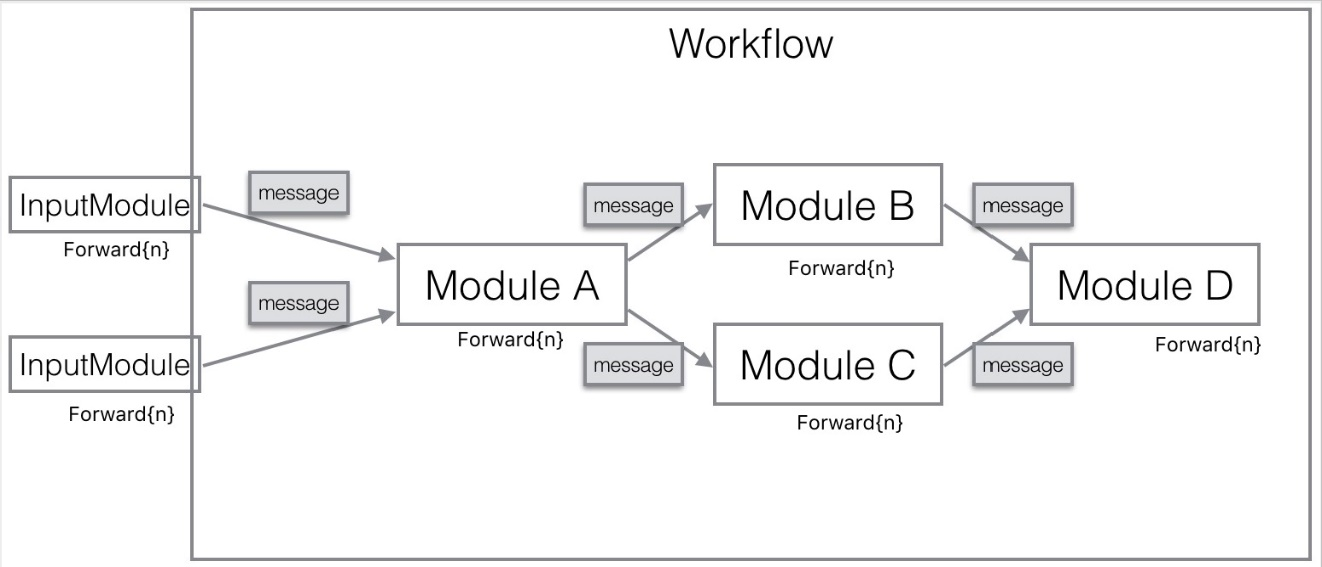
\includegraphics[width=8cm]{img/workflow.png}
	\bicaption{基于模块构造工作流}{Workflow based on module construction}
	\label{基于模块构造工作流}
\end{figure}

基于深度学习的视觉算法,其计算部分流程可以概括为前处理、模型推理和后处理三个阶段。前处理阶段通常包括图像缩放、归一化、裁剪、色彩空间转换等,这些操作需要以图像数据为输入,输出符合模型输入要求的张量数据,根据设计定位,可以封装为算子(Operator),也可以封装为计算图中的一个模块节点(Module)\ref{模块的基本结构}。后处理阶段通常包括后验概率转换、非极大值抑制、边框回归、关键点检测等操作,用于进一步优化模型的结果,这些操作也通常可以实现为计算图中的模块。

模型推理阶段是计算图中的核心部分,内部包括卷积、池化、全连接等多种结构,以及激活函数、归一化、Dropout\cite{srivastava2014dropout}等,每个节点都接受上一层的输出作为输入,输出结果经过下一层的处理,最终得到模型的分类或回归结果。但在模型的部署阶段,我们一般只会把模型作为一个端到端的模块来考虑,关注其吞吐量和计算延迟,而不会过度探索其内部的细节。

需要注意的是,用于推理计算的模块不一定只有一个,真实的业务部署场景有多个推理模型同时运行非常常见,对于同种推理则会通过构造批次处理(Batch Forward)\cite{mcclelland1987parallel}以达到GPU(ASIC)的计算和带宽上限。此外,虽然专用硬件非常适合这一计算任务,少量情况下也会选择在CPU上运行。

完整考虑\ref{计算机视觉算法模型的部署外环境}描述的部署外环境,模块的抽象还应该纳入IO部分。常见的IO模块一般用来处理传感器设备的数据收发,例如不同的实例化IO模块和各种规格设备的摄像机,磁盘设备,网络套接字一一对应,生成具体的节点。无论作为输入还是输出,虽然没有具体的计算任务,但仍然需要进行完整的操作执行,因此同样应该提供对应的时间戳信息和附属的元信息。模块并不一定由单一的进程启动,例如负责发送数据的IO模块(负责管理某一相机设备的输入数据),其完全可以单独运行,通过RPC的网络数据传输方式和计算图的其他节点通讯。基于这个前提,封装模块可能涉及多重实现语言(python,c++.etc.)和多个进程之间的数据通讯。

\begin{figure}[htbp]
	\centering
	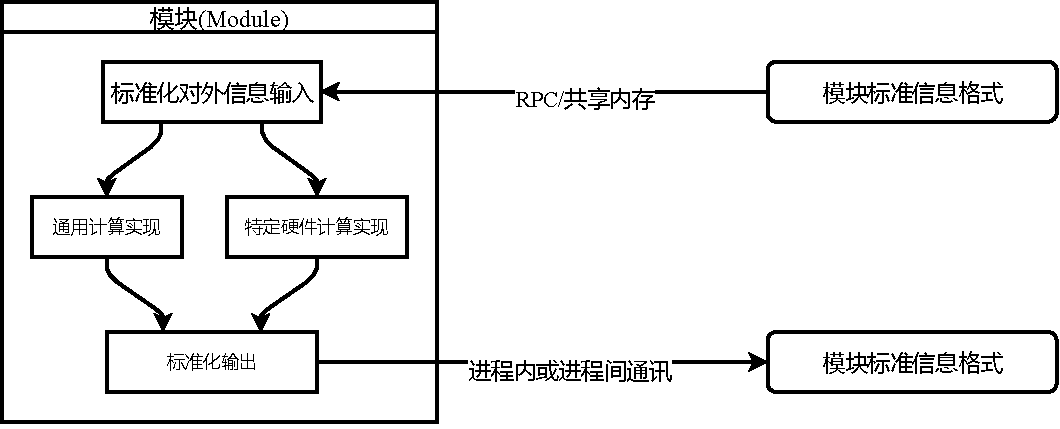
\includegraphics[width=8cm]{img/module.pdf}
	\bicaption{模块的基本结构}{The basic structure of the module}
	\label{模块的基本结构}
\end{figure}


\subsection{计算机视觉算法的部署延迟测量}\label{计算机视觉算法的部署延迟测量}
\subsubsection{计算机视觉算法延迟的提取方式}\label{计算机视觉算法延迟的提取方式}
计算机视觉算法的部署延迟,通常是指从输入图像/视频,到算法产生输出结果所需的时间。当以计算图的模块为单位,对整个算法执行过程中做出抽象的过程中,整个流程的调用关系已经确定。这意味着对延迟的测量并非只能和传统的服务端相同,粗略的计算端到端的时间开销,而是可以针对整个完整的计算机视觉算法运行流程,逐环节拆分为单步延迟,以此来提供整体的观测能见度。

和一般基于CPU的计算任务不同,计算机视觉算法模块之间一般根据功能特点切分,但不同节点,尤其是负责模型推理的模块,其工作负载明显超出一个数量级。如果对整体时延求和,则推理模块的权重占比过高,导致其他模块的性能优化点不易发现。例如推理延迟的具体数值,取决于使用的算法和实际的硬件设备。一般来说,现代GPU上执行一个pytorch直接生成的TorchScript模型,中等参数规模(例如RetinaNet\cite{lin2017focal})的神经网络模型,推理延迟大致在几十个毫秒。经过TensorRT的量化(Quantization),可以实现在精度下降个位数百分点的范围内,减少超过50$\%$的推理延迟,而单个前,后处理算子,基本在1-2ms的左右。但对于算子细节的实现优化并非没有意义,因为对于计算机视觉算法的部署而言,每一个算子都属于需要持续重复执行的热点路径(Hot Path), 如何对这些常用计算函数的效率进行优化,也是学术界一直讨论课题\cite{cai2019maxpoolnms}。

而基于编译器层提供的性能观测工具(Nsight Compute,Intel VTune\cite{reinders2005vtune}),其切分的粒度一般以函数为单位,依赖于函数的符号表(Symbol Table),其通过火焰图(Flame Graph)\cite{gregg2016flame}等方式进行可视化分析,帮助程序的使用者查找优化节点性能。这种方式的缺点在于颗粒度太小,如果以函数为单位,会需要记录海量的延迟信息,并且实时观测的开销太高,资源不足的情况下会影响算法本身的运行。
\begin{figure}[htbp]
	\centering
	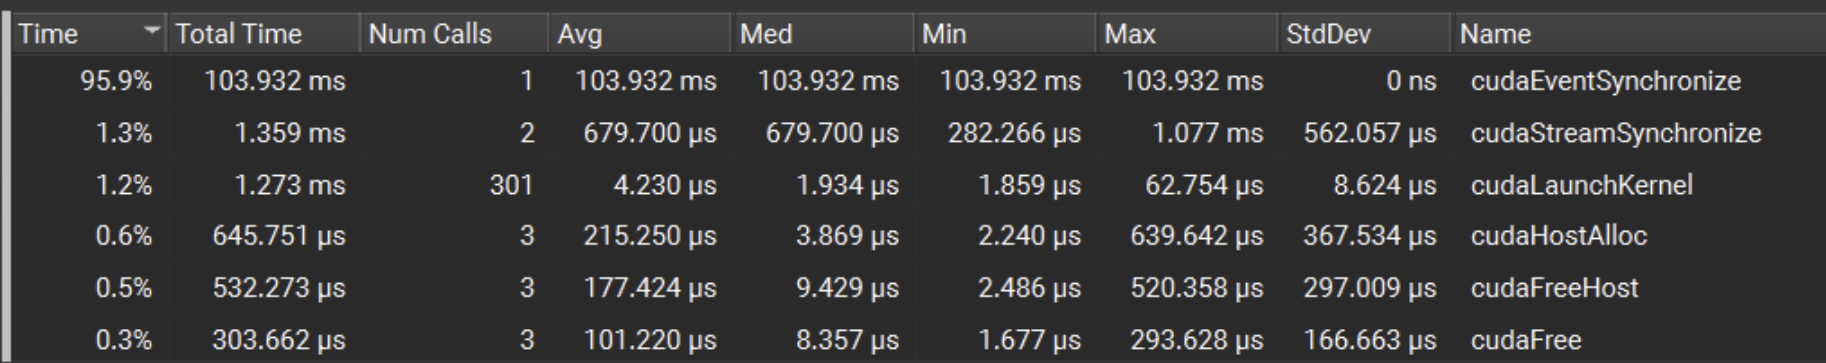
\includegraphics[width=8cm]{img/nsight_func.png}
	\bicaption{Nsight Compute的观测结果:颗粒度依赖于函数符号}{
		Nsight Compute Observations: Granularity Depends on Function Symbol}
	\label{NsightCompute的观测结果}
\end{figure}


因此,论文设计了一种基于阶段(Stage)选择的算法延迟测量方式,既考虑到观测能见度,也权衡了实时观测系统的低负载需求。具体的,以模块为时间戳获取的最小单位,一个阶段内可以放置多个模块。至少需要在一个阶段首个模块进入点,和最后一个模块的结束点,触发延迟的记录事件,捕获时间戳和上下文信息,并提交到专用的日志记录工具。

一般的场景下,对于由多个视觉算法组成的业务模型,数据所需要经过的环节和顺序都是固定的,其运行的整个流程具有一个树形的拓扑结构,获取一个观测的阶段,有两种不同的方式,对整个路径进行划分,由于整体是一个有向无环图,因此选择的阶段可能存在分支,也可能是无分叉的连续模块。对于一段无分支的区间,可以任意选择连续的模块构造一个或多个"阶段",当一个区间存在分支,由于我们一般认为,同一个模块处理的计算任务是等价的(近似于无状态函数,数据处理的开销和数据的来源无关),因此对重合的路径,应该切分处理,具体的,即一个阶段的选择,不能跨越产生分支的节点(可以作为端点),应该阶段分叉前的部分,重新在后续路径上构造新的阶段。

\begin{figure}[htbp]
	\centering
	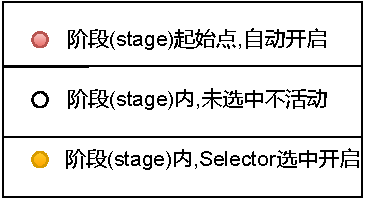
\includegraphics[width=8cm]{img/trace_l.pdf}
	\bicaption{论文观测机制示意图图例}{Schematic illustration of the observation mechanism in this thesis}
	\label{论文观测机制示意图图例}
\end{figure}

\begin{figure}[htbp]
	\centering
	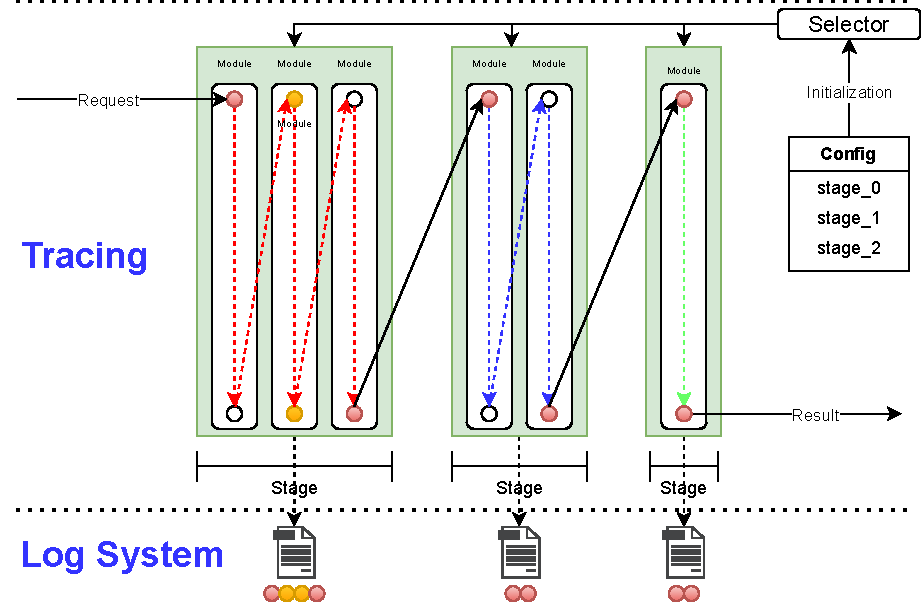
\includegraphics[width=12cm]{img/trace.pdf}
	\bicaption{论文观测机制示意图}{Schematic diagram of the observation mechanism in this thesis}
	\label{论文观测机制示意图}
\end{figure}

最终对于延迟提取方式的描述,是一系列以阶段为分区的延迟数据采集关系,这种构造过程无需修改代码本身,而是通过外部的配置文件(Config)。系统运行之前,会先实例化一个选择器(Selector),选择器通过读取配置文件的信息,确定阶段的划分方式,然后启动阶段两段模块上的内部设置为开启的观测点\cite{论文观测机制示意图}。这一机制依赖于操作系统内核的动态观测技术,具体实现在ref的环节会详细讨论。但可以概括为,在每个模块的出,入口上放置的观测节点,是通过选择器(Selector)的启动后才具有触发延迟记录事件的功能,否则仅相当于一条不产生作用的空指令,不会导致额外的性能开销。

每一个阶段的延迟会被归档记录到一个日志中,通过获得开启的采样点时间戳,若对于单个模块,则开启和结束时间时间戳的差值就是模块的执行延迟,而到达下一个模块开启之前的时间,则可以视为调度和模块间的通讯延迟。这种情况下,不一定要选择阶段中全部的采样点,例如同一个进程地址空间之内的小计算模块之间的通讯和调度,大部分时候都没有观测的必要。


通过这一方式,可以灵活的控制观测的颗粒度,获取数据的详细程度取决于具体的需求。在软件的优化阶段,可以只选择前处理,后处理等部分的模块,避免推理模块的时延占比过高,不利于具体发现可以优化的模块,对比优化后的结果,可以只选择单一模块即可。运行时,延迟主要是用于事后的故障追踪,此时更多关注的硬件的情况,以外部传输,CPU侧,GPU(ASIC)侧来做大颗粒度划分,运行在同一硬件的连续模块直接归档到同一个阶段,减少产生的日志事件,降低观测的性能开销。

设计这种阶段选择的模式,实际生产中一个极大的便利点在于解除了业务软件本身和观测延迟部分的耦合,因为这种通过选择器去开启观测点的使用方式,并不会对软件目标运行产生影响,换而言之,采样和分析不会让被观测的对象所感知。这种方式构造了一种"热插拔"和"低耦合",即采样和分析的工具是完全独立于生产系统,工具何时进行采样,何时和怎样进行统计分析,取决于工具的开发者和使用者。这使得测试不同模块的性能,只需要修改生成观测选择的配置文件,而不需要类似注入日志的方式,哪怕调整输出格式都需要直接重新修改和编译。并且"按需采集"的方式使得观测者对于软件的性能负载可以调节和控制,一种机制即可适配运行时和发布前不同的延迟观测需求。

\subsubsection{计算机视觉算法部署中的延迟元数据}\label{计算机视觉算法部署中的延迟元数据}
\paragraph{延迟相关元数据}
当模块中的采样点触发延迟观测事件,获得此时的时间戳的同时,额外的程序状态信息,即论文所定义的延迟元数据。元数据通常被定义为描述数据的数据,对于延迟而言,即一些和延迟相关的状态信息,包括硬件状态和软件状态。

模块是一种对于底层实现的抽象,而硬件状态则指的是实际执行这一模块的物理环境,例如CPU/GPU/ASIC(Neural Network Processing Unit,NPU)的工作状态。以CPU侧的运行为例,一般包括内存占用(Memory Usage),CPU当前频率,当前CPU上等待执行的队列长度等信息。而对于负责神经网络推理,和部分特殊的前后处理计算的专用硬件(GPU/NPU)而言,由于其实现的体系结构非常多样化,其观测的指标更多取决于硬件驱动直接提供的定量评估值,例如设备利用率,显存占用等。部分嵌入式环境下运行的硬件还会提供一些特殊的状态信息来辅助调试,例如NPU部分的电压值,常用于功耗分析和故障调试等场景。

软件状态信息则主要包括程序的上下文,一般包括程序当前所属的进程、线程ID,以及一些运行时产生的变量,一般还会根据需求,选择函数的参数堆栈,调用栈信息等。如何利用这些信息相当自由,甚至于可以根据一些特殊需求生成一些额外的信息。

这些额外信息是衡量可靠性的关键参考,获取元数据的能力,是观测系统中能见度的直观体现。本文拓展计算机视觉算法可观测维度的方式,就是利用软件的状态信息去制作延迟数据之间的钩子(Hook),而事后追踪的故障定位,也非常依赖于这些元数据信息。
\paragraph{使用元数据拓展观测维度}
一般的服务端的观测工具,主要关注单一维度分析。例如最常见的是系统负载观测程序。举例iostat\cite{chandran2014monitoring},主要用于监控系统设备的IO负载情况,用户可以通过指定统计的次数和时间来获得所需的统计信息,类似平均请求扇区的大小,平均请求队列的长度,每秒读/写的扇区数(rsec/wsec)等。这种观测一般仅限某个单独的维度,具体来说,这种观测类似于对系统运行某一个环节,进行横向的截面采样,统计的指标一般是同类数值的平均值/最大值/最小值等分布信息。

一部分原因是因为这些工具诞生于早期的UNIX,设计核心理念之一是"一个工具只做一件事,但要做好",每个工具通过标准输入和输出进行协作,从而实现高度的可组合性和可重用性,但这一方式如今已经有较大的局限性,以此方式实现更高的观测可见度工作量太大,同时只能做到事后分析,无法做到运行时处理。

在计算机视觉算法的延迟数据观测中,我们重点提到了使用传统方式,观测维度不足的问题\ref{论文研究的出发点},这和现代软件工程的多层次导致的复杂性是类似的,简单的日志输出或者单一环节负载观测, 由于信息不足(采样的数据只服务于统计指标),很难在多个模块或层次之间建立联系,或者无法做到运行时建立。例如上述采样点所获得的时间戳数据,即便了解采样点的位置,但无法判断延迟具体归属于哪一份数据,举例而言,上文所描述的构造阶段,就是以时间的维度,考虑每一张图片具体在每个环节上的时间开销。这种纵向观测维度是非常有意义的,尤其针对之前所描述的"延迟窗口期"问题,以及这种方式可以非常清晰的体现出数据和计算之间的关系,而不会因为平均值等统计的原因被抹平。

本文实现这种跨越阶段的数据联系,是通过以一些元数据作为数据之间匹配的唯一键,通过哈希表这一数据结构,创造一些延迟数据之间的钩子(Hook),这一实现方式深度依赖操作系统内核新特性的支持,在ref中会做具体介绍。

\section{计算机算法的延迟观测意义}\label{计算机算法的延迟观测意义}
\subsection{计算图调度参考}\label{计算图调度参考}
计算图调度是指对计算图中的操作进行排序和调度,以便在计算中最大化利用资源并最小化延迟。这通常涉及将依赖关系转化为并发操作和数据流,并将操作分配到可用的计算资源上。常用的技术是基于有向无环图(Directed Acyclic Graph,DAG)的调度算法,在对各个模块的依赖关系确定后,将DAG中的节点排序,以便操作可以按照正确的顺序执行。可以使用拓扑排序算法来实现。将操作分配给可用的计算资源,以最大化并发性, 在分配资源后,需要将操作调度到实际的计算资源上,例如GPU,CPU,ASIC。这通常涉及将操作映射到适当的设备上,并将其分配到可用的计算资源中。

对于前处理和后处理阶段,应该根据具体的应用场景来选择使用CPU还是专用硬件进行计算。CPU的优点是具有较强的通用性和灵活性,能够适应各种不同的计算任务,具有较高的单线程执行性能,在处理一些计算较少、但需要高并发处理的任务时比较优秀。一般的,由于CPU资源普遍更加富余,且前后处理需要对接外部新信息的输入输出,涉及到网络和IO的场景,因此大部分情况下会派发到CPU,少数边缘计算的硬件,其内存和专用计算硬件的显存在主板上可以直连,拷贝代价较低,则会使用专用算子进行执行,这些细节对会被封装在模块执行的内部。

由于对于一个固定功能的模块,在不考虑线程切换的开销下,需要执行的计算任务完全相同,因此理论上单个计算节点通过一份数据的时间应该会在一个相对稳定的范围内波动。在这种前提下,延迟信息可以近似等价于工作负载,作为计算图调度的重要参考依据。然而由于针对不同的硬件情况,以及软件的支持情况,模块的实现方式都是不同的,虽然可以提供具有一致的接口,但实际上运行的表现会有较大的差异。一个典型的例子就是部署过程中对于模型的量化,这种技术将浮点型参数和激活值转换为低位宽的整数类型,从而在不显著降低模型精度的情况下减小模型的存储和计算开销。由于量化后的计算需要更少的存储空间和计算资源,因此可以显著降低模型推理的延迟。量化后不仅减少了存储和带宽的需求,同时整数计算还大幅度的减少了计算开销,由于现代硬件加速器通常采用定点计算,因此量化可以更好地适配这些硬件,从而显著提高计算性能。这会使得即便是理论上最稳定的推理部分,实际部署的过程也会因为精度的需求不同,表现出完全不同的延迟。至于算子则取决于硬件的支持以及实现的完成度。

\begin{figure}[htbp]
	\centering
	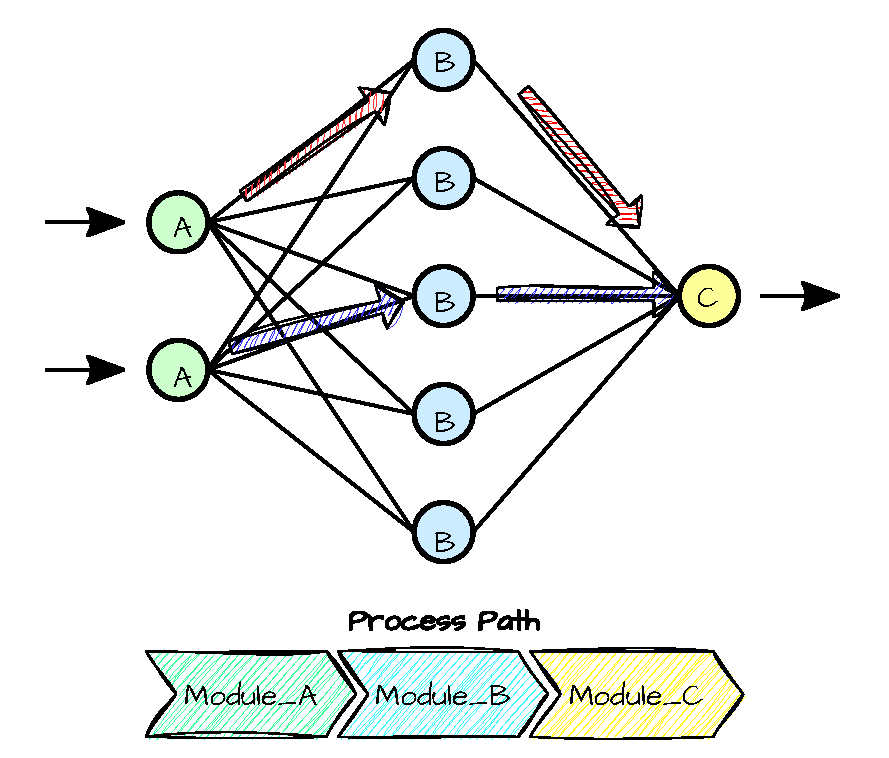
\includegraphics[width=8cm]{img/path.pdf}
	\bicaption{红蓝不同路径在计算图中通过相同的模块}{Different Red and blue paths pass through the same modules in the computation graph}
	\label{ABCpath}
\end{figure}


虽然延迟可以近似理解为在特定资源上的工作负载,但是在ARM硬件中,CPU存在大小核的情况,即某些处理器有一些性能更高的大核心和一些性能较低的小核心。对于一个相同计算负载的任务,例如一个前处理任务,在大核心上会具有更小的延迟,移动端推理框架比如ncnn和paddlelite等框架\cite{febvay2020low}就提供了运行时功耗级别的设置,实质上就是通过绑定大核实现高功耗模式,绑定小核实现低功耗模式。最好的情况下,我们还希望能捕获这种更细致颗粒度的信息作为优化参考,但参考\ref{现有计算机视觉算法延迟观测的一般方法与不足}所描述的一般日志系统,这类元信息的获取就性能负载而言并不廉价。

\begin{figure}[htbp]
	\centering
	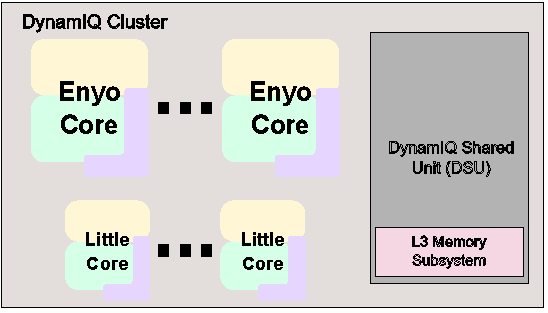
\includegraphics[width=8cm]{img/arm.pdf}
	\bicaption{ARM A76的大小核架构\cite{arm76}}{ARM big.LITTLE architecture of A76}
	\label{ARM的大小核架构}
\end{figure}

因此,延迟的观测数据可以作为一种重要的优化参考存在,但不是一个确定的常数,而是需要根据具体的部署状态去进行测量,一个颗粒度可以自由控制的延迟观测系统,在优化阶段可以发挥相当多的作用。

\subsection{优化参数设置}\label{优化参数设置}
部分参数的设定也会影响系统的性能,一个比较常见的指标是线程池的大小设置,线程池是一种用于管理和调度线程的技术,可以有效地利用系统资源,提高系统的性能和响应速度。对于计算机视觉任务来说,其关键瓶颈通常在模型推理部分,要尽可能的减少其等待时间。线程池可以预先创建一定数量的线程,每当获得模型的输出,快速为推理模块填充新的输入。视觉算法通常需要处理大量的图像和视频数据,需要大量的并发和并行,因此线程池可以带来良好的重用,减少线程的创建和销毁造成的系统负荷,但也需要根据具体的应用场景来进行评估和调整,例如根据延迟信息代表的工作负载,避免设定太多的线程造成过多上下文切换过多,同时也应该考虑内存占用的问题,这一点在嵌入式系统的边缘计算中尤其重要\cite{threadpool}。

\begin{figure}[htbp]
	\centering
	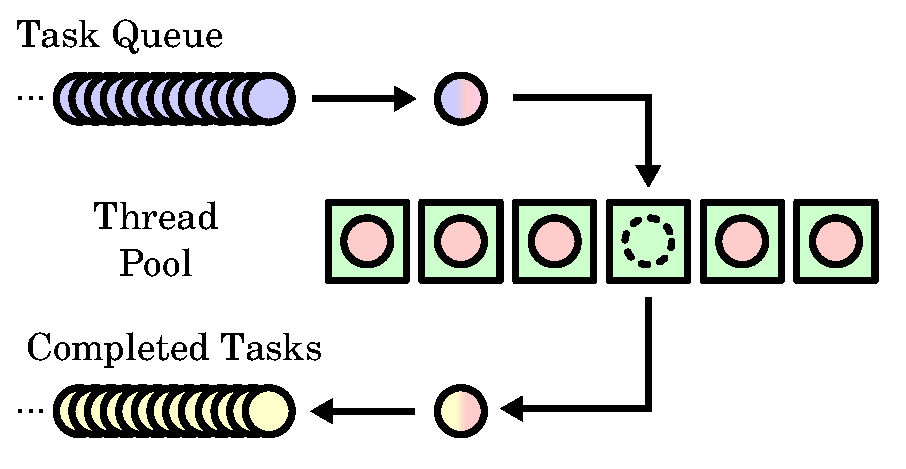
\includegraphics[width=8cm]{img/thread_pool.pdf}
	\bicaption{线程池的工作过程}{The working process of thread pool}
	\label{线程池的工作过程}
\end{figure}

在延迟的观测可以不止存在一个维度,对于\ref{基于计算图的模块抽象}中的推理模块,其运行的延迟可以进行数据分布的统计,考察同一类模块执行计算任务时间开销的变化情况,也可以选择根据以数据本身为观测维度,即数据从进入计算机视觉算法系统开始,到获得对应的结果信息对应在每个环节的延迟开销。这当中必然还存在一些等待时间,例如在线程池中排队等待响应,以及对应线程在CPU上经过的上下文切换数量。如果等待时间占比太长,发生的线程调度过于频繁,则说明线程池设置的规模太大,参数配置并不合理。

\subsection{事后追踪参考}\label{事后追踪参考}
日志的事后追踪能力是指在程序运行过程中,将程序的关键信息和状态记录下来,并保存到日志中,以便在程序出现问题或异常时,能够通过分析日志来查找问题和排除故障。计算机视觉算法在运行时的延迟信息,以及一些附带的元数据,包括时间戳、线程ID、进程ID、运行环境,以及可以控制颗粒度的,具体在哪一个模块运行这样用来描述程序执行路径的上下文信息。这样的筛查能力可以在端到端的总体延迟出现波动时,可以快速排查到出现故障的模块,提供一种可定位性。

大部分边缘业务因为数据和安全性的考虑,基本只在内网环境,本质上在离线状态下进行长时间运行。当出现一些偶发的故障,需要排查和处理,由于嵌入式系统的部署特点,一般只能通过对历史故障的描述,至少在几个小时或者几天后,先将服务下线,然后才能开始尝试复现故障问题,这种重现由于缺少参考信息,一般非常困难。

\begin{figure}[htbp]
	\centering
	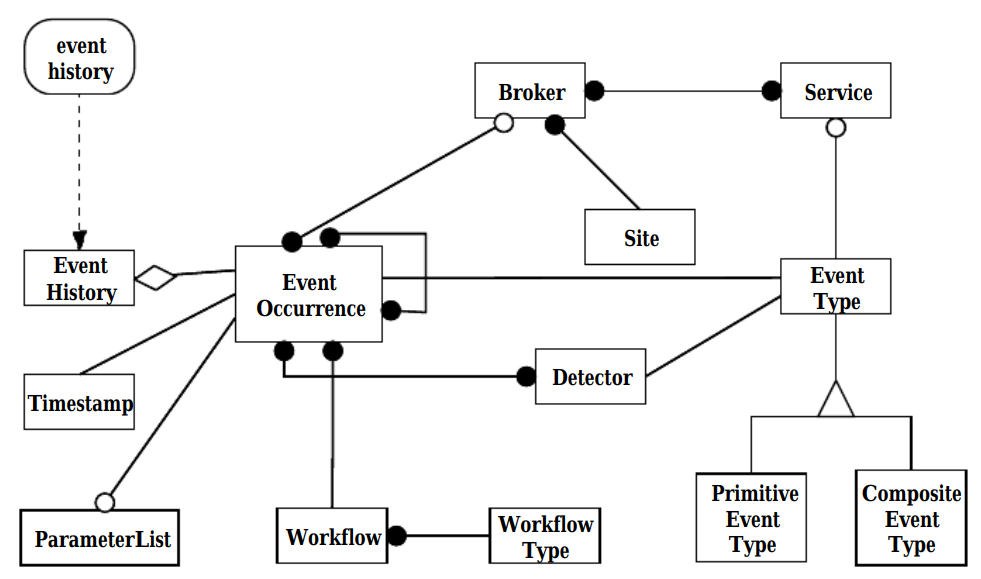
\includegraphics[width=8cm]{img/eve.png}
	\bicaption{一种日志事件跟踪的设计方法\cite{geppert1997logging}}{
		A Design Method for Logging Event Tracing}
	\label{一种日志事件跟踪的设计方法}
\end{figure}

事后追踪能力主要就是为这一情况提供帮助,记录一些额外的参考信息。本文讨论的延迟数据,一个重要作用,就是可以通过延迟数据日志来定位故障发生的时间点,以及根据延迟出现异常波动的具体环节,推测故障发生在运行中的位置\cite{geppert1997logging}。特别的,延迟的元信息,即软件硬件的状态信息,由于是一种"活体观测"的运行时数据,因此非常宝贵,相当于不需要重现故障,就可以获得事件发生时的关键信息。

\section{本章总结}\label{本章总结}
本章的主要目的是定义问题,明确需求。延迟作为一个两端时间戳的差值,首先需要明确测量的具体方式。本章首先描述了基于计算图和模块封装,来定义和实现计算机视觉算法部署的一般方法,之后具体描述了基于选择器和采样点的设计方案,阐述了算法延迟的提取过程,并对技术选型进行分析,最后探讨了记录延迟数据在计算机视觉算法部署工程中的作用。

\chapter{轻量级视觉算法部署延迟观测系统实现}

\section{延迟观测事件构造}
\ref{基于计算图的模块抽象}描述了一个计算机视觉算法在部署过程中,一种工程上的封装方式。即业务流程可以被封装成多个模块的组合,通过对模块的串联实现并行和并发控制,而框架,硬件,实现上的兼容性被封装在模块的具体内部实现当中。
\ref{计算机视觉算法延迟的提取方式}描述了基于上述封装,论文所描述的计算机视觉算法延迟的提取方式。其核心思路是将对延迟的观测功能外置,实现为独立的工具。基于设置阶段这一概念,允许通过配置和修改文本config的方式,选择具体启动模块上的哪些采样点来工作,实现了业务软件的运行和观测本身解耦。
"热插拔"和"低耦合"的方式,不仅在延迟收集的过程中带来了便利性,避免反复编译程序主体,同时,在边缘计算的嵌入式场景下,"按需采集"的延迟提取有效的限制了实时观测程序对算法吞吐和响应时间的影响。
论文所述方案是一种基于事件(event)的响应机制,而其良好的性能表现则是依赖于操作系统使能的动态追踪技术。本章节从延迟观测事件的构造开始论述,进而介绍了如何获取完整的延迟信息和赢软件状态信息,以及最终如何跨越用户态和内核态获得结果。
\subsection{动态追踪技术概述}
动态追踪技术(Dynamic Tracing)是一种后现代的调试技术,其诞生动机就是面对更加复杂的观测场景,提高对于整个生产系统的可观测能见度和控制力,和ref所描述的早期Unix工具不同,其强调对于开发人员的高度可拓展性,是一种近似于运行时调试的能力。


\begin{acknowledgement}
\shtthesis{} 派生于中国科学院大学论文模板 \textsf{ucasthesis}\footnote{\url{https://github.com/mohuangrui/ucasthesis},使用 GPLv3 许可证分发。};v0.2.0 开发过程中参考了清华大学论文模板 \textsf{thuthesis}\footnote{\url{https://www.ctan.org/pkg/thuthesis},使用 LPPL-1.3c 许可证分发。},特别是 \verb|\thusetup| 命令的设计和实现;v0.3.0 及后续版本开发过程中参考了复旦大学论文模板 \textsf{fduthesis}\footnote{\url{https://www.ctan.org/pkg/fduthesis},使用 LPPL-1.3c 许可证分发。},以及其超链接配色方案。这些项目中流淌的智慧,以及项目作者们的专业态度和共享精神使得 \shtthesis{} 的开发及完善成为可能。
\end{acknowledgement}
\makebiblio
\ifgraduate
\begin{resume}
  李润东,\shtthesis{} 项目初版作者及维护者,热爱摸鱼。
\end{resume}

\begin{publications}
  论文发表…… (非匿名环境)
\end{publications}

\begin{publications*}
  论文发表…… (匿名环境)
\end{publications*}

\begin{patents}
  专利申请或授权记录…… (非匿名环境)
\end{patents}

\begin{patents*}
  专利申请或授权记录…… (匿名环境)
\end{patents*}

\begin{projects}
  个人参与的科研项目、获奖情况…… (仅非匿名环境显示)
\end{projects}
\fi

\end{document}
